% Options for packages loaded elsewhere
\PassOptionsToPackage{unicode}{hyperref}
\PassOptionsToPackage{hyphens}{url}
\PassOptionsToPackage{dvipsnames,svgnames,x11names}{xcolor}
%
\documentclass[
  ignorenonframetext,
]{beamer}
\usepackage{pgfpages}
\setbeamertemplate{caption}[numbered]
\setbeamertemplate{caption label separator}{: }
\setbeamercolor{caption name}{fg=normal text.fg}
\beamertemplatenavigationsymbolsempty
% Prevent slide breaks in the middle of a paragraph
\widowpenalties 1 10000
\raggedbottom

\usepackage{amsmath,amssymb}
\usepackage{iftex}
\ifPDFTeX
  \usepackage[T1]{fontenc}
  \usepackage[utf8]{inputenc}
  \usepackage{textcomp} % provide euro and other symbols
\else % if luatex or xetex
  \usepackage{unicode-math}
  \defaultfontfeatures{Scale=MatchLowercase}
  \defaultfontfeatures[\rmfamily]{Ligatures=TeX,Scale=1}
\fi
\usepackage{lmodern}
\usetheme[]{AnnArbor}
\usecolortheme{dolphin}
\usefonttheme{structurebold}
\ifPDFTeX\else  
    % xetex/luatex font selection
\fi
% Use upquote if available, for straight quotes in verbatim environments
\IfFileExists{upquote.sty}{\usepackage{upquote}}{}
\IfFileExists{microtype.sty}{% use microtype if available
  \usepackage[]{microtype}
  \UseMicrotypeSet[protrusion]{basicmath} % disable protrusion for tt fonts
}{}
\makeatletter
\@ifundefined{KOMAClassName}{% if non-KOMA class
  \IfFileExists{parskip.sty}{%
    \usepackage{parskip}
  }{% else
    \setlength{\parindent}{0pt}
    \setlength{\parskip}{6pt plus 2pt minus 1pt}}
}{% if KOMA class
  \KOMAoptions{parskip=half}}
\makeatother
\usepackage{xcolor}
\newif\ifbibliography
\setlength{\emergencystretch}{3em} % prevent overfull lines
\setcounter{secnumdepth}{-\maxdimen} % remove section numbering

\usepackage{color}
\usepackage{fancyvrb}
\newcommand{\VerbBar}{|}
\newcommand{\VERB}{\Verb[commandchars=\\\{\}]}
\DefineVerbatimEnvironment{Highlighting}{Verbatim}{commandchars=\\\{\}}
% Add ',fontsize=\small' for more characters per line
\usepackage{framed}
\definecolor{shadecolor}{RGB}{241,243,245}
\newenvironment{Shaded}{\begin{snugshade}}{\end{snugshade}}
\newcommand{\AlertTok}[1]{\textcolor[rgb]{0.68,0.00,0.00}{#1}}
\newcommand{\AnnotationTok}[1]{\textcolor[rgb]{0.37,0.37,0.37}{#1}}
\newcommand{\AttributeTok}[1]{\textcolor[rgb]{0.40,0.45,0.13}{#1}}
\newcommand{\BaseNTok}[1]{\textcolor[rgb]{0.68,0.00,0.00}{#1}}
\newcommand{\BuiltInTok}[1]{\textcolor[rgb]{0.00,0.23,0.31}{#1}}
\newcommand{\CharTok}[1]{\textcolor[rgb]{0.13,0.47,0.30}{#1}}
\newcommand{\CommentTok}[1]{\textcolor[rgb]{0.37,0.37,0.37}{#1}}
\newcommand{\CommentVarTok}[1]{\textcolor[rgb]{0.37,0.37,0.37}{\textit{#1}}}
\newcommand{\ConstantTok}[1]{\textcolor[rgb]{0.56,0.35,0.01}{#1}}
\newcommand{\ControlFlowTok}[1]{\textcolor[rgb]{0.00,0.23,0.31}{\textbf{#1}}}
\newcommand{\DataTypeTok}[1]{\textcolor[rgb]{0.68,0.00,0.00}{#1}}
\newcommand{\DecValTok}[1]{\textcolor[rgb]{0.68,0.00,0.00}{#1}}
\newcommand{\DocumentationTok}[1]{\textcolor[rgb]{0.37,0.37,0.37}{\textit{#1}}}
\newcommand{\ErrorTok}[1]{\textcolor[rgb]{0.68,0.00,0.00}{#1}}
\newcommand{\ExtensionTok}[1]{\textcolor[rgb]{0.00,0.23,0.31}{#1}}
\newcommand{\FloatTok}[1]{\textcolor[rgb]{0.68,0.00,0.00}{#1}}
\newcommand{\FunctionTok}[1]{\textcolor[rgb]{0.28,0.35,0.67}{#1}}
\newcommand{\ImportTok}[1]{\textcolor[rgb]{0.00,0.46,0.62}{#1}}
\newcommand{\InformationTok}[1]{\textcolor[rgb]{0.37,0.37,0.37}{#1}}
\newcommand{\KeywordTok}[1]{\textcolor[rgb]{0.00,0.23,0.31}{\textbf{#1}}}
\newcommand{\NormalTok}[1]{\textcolor[rgb]{0.00,0.23,0.31}{#1}}
\newcommand{\OperatorTok}[1]{\textcolor[rgb]{0.37,0.37,0.37}{#1}}
\newcommand{\OtherTok}[1]{\textcolor[rgb]{0.00,0.23,0.31}{#1}}
\newcommand{\PreprocessorTok}[1]{\textcolor[rgb]{0.68,0.00,0.00}{#1}}
\newcommand{\RegionMarkerTok}[1]{\textcolor[rgb]{0.00,0.23,0.31}{#1}}
\newcommand{\SpecialCharTok}[1]{\textcolor[rgb]{0.37,0.37,0.37}{#1}}
\newcommand{\SpecialStringTok}[1]{\textcolor[rgb]{0.13,0.47,0.30}{#1}}
\newcommand{\StringTok}[1]{\textcolor[rgb]{0.13,0.47,0.30}{#1}}
\newcommand{\VariableTok}[1]{\textcolor[rgb]{0.07,0.07,0.07}{#1}}
\newcommand{\VerbatimStringTok}[1]{\textcolor[rgb]{0.13,0.47,0.30}{#1}}
\newcommand{\WarningTok}[1]{\textcolor[rgb]{0.37,0.37,0.37}{\textit{#1}}}

\providecommand{\tightlist}{%
  \setlength{\itemsep}{0pt}\setlength{\parskip}{0pt}}\usepackage{longtable,booktabs,array}
\usepackage{calc} % for calculating minipage widths
\usepackage{caption}
% Make caption package work with longtable
\makeatletter
\def\fnum@table{\tablename~\thetable}
\makeatother
\usepackage{graphicx}
\makeatletter
\def\maxwidth{\ifdim\Gin@nat@width>\linewidth\linewidth\else\Gin@nat@width\fi}
\def\maxheight{\ifdim\Gin@nat@height>\textheight\textheight\else\Gin@nat@height\fi}
\makeatother
% Scale images if necessary, so that they will not overflow the page
% margins by default, and it is still possible to overwrite the defaults
% using explicit options in \includegraphics[width, height, ...]{}
\setkeys{Gin}{width=\maxwidth,height=\maxheight,keepaspectratio}
% Set default figure placement to htbp
\makeatletter
\def\fps@figure{htbp}
\makeatother
% definitions for citeproc citations
\NewDocumentCommand\citeproctext{}{}
\NewDocumentCommand\citeproc{mm}{%
  \begingroup\def\citeproctext{#2}\cite{#1}\endgroup}
\makeatletter
 % allow citations to break across lines
 \let\@cite@ofmt\@firstofone
 % avoid brackets around text for \cite:
 \def\@biblabel#1{}
 \def\@cite#1#2{{#1\if@tempswa , #2\fi}}
\makeatother
\newlength{\cslhangindent}
\setlength{\cslhangindent}{1.5em}
\newlength{\csllabelwidth}
\setlength{\csllabelwidth}{3em}
\newenvironment{CSLReferences}[2] % #1 hanging-indent, #2 entry-spacing
 {\begin{list}{}{%
  \setlength{\itemindent}{0pt}
  \setlength{\leftmargin}{0pt}
  \setlength{\parsep}{0pt}
  % turn on hanging indent if param 1 is 1
  \ifodd #1
   \setlength{\leftmargin}{\cslhangindent}
   \setlength{\itemindent}{-1\cslhangindent}
  \fi
  % set entry spacing
  \setlength{\itemsep}{#2\baselineskip}}}
 {\end{list}}
\usepackage{calc}
\newcommand{\CSLBlock}[1]{\hfill\break\parbox[t]{\linewidth}{\strut\ignorespaces#1\strut}}
\newcommand{\CSLLeftMargin}[1]{\parbox[t]{\csllabelwidth}{\strut#1\strut}}
\newcommand{\CSLRightInline}[1]{\parbox[t]{\linewidth - \csllabelwidth}{\strut#1\strut}}
\newcommand{\CSLIndent}[1]{\hspace{\cslhangindent}#1}


% logo
\titlegraphic{
\includegraphics[width=4cm]{../000_logos/logo-blue-vertical}}
\logo{\ifnum\thepage>1
\includegraphics[width=0.5cm]{../000_logos/logo-blue-vertical}\fi}

% UMNG: Manual de image institucional

% Colors

% Umng
\definecolor{yellow}{HTML}{fdc600}
\definecolor{red}{HTML}{ee2a24}

% Estudios a Distancia
\definecolor{blue1}{HTML}{12245b}
\definecolor{blue2}{HTML}{767ca6}
\definecolor{blue3}{HTML}{cad2ec}

% Modify items
\setbeamercolor{palette primary}{bg=blue3}
\setbeamercolor{palette tertiary}{bg=blue1}
\setbeamercolor{frametitle}{bg=yellow}

% Hyperlinks
\hypersetup{
  linkcolor=red,
  citecolor=red
}

\makeatletter
\@ifpackageloaded{caption}{}{\usepackage{caption}}
\AtBeginDocument{%
\ifdefined\contentsname
  \renewcommand*\contentsname{Table of contents}
\else
  \newcommand\contentsname{Table of contents}
\fi
\ifdefined\listfigurename
  \renewcommand*\listfigurename{List of Figures}
\else
  \newcommand\listfigurename{List of Figures}
\fi
\ifdefined\listtablename
  \renewcommand*\listtablename{List of Tables}
\else
  \newcommand\listtablename{List of Tables}
\fi
\ifdefined\figurename
  \renewcommand*\figurename{Figure}
\else
  \newcommand\figurename{Figure}
\fi
\ifdefined\tablename
  \renewcommand*\tablename{Table}
\else
  \newcommand\tablename{Table}
\fi
}
\@ifpackageloaded{float}{}{\usepackage{float}}
\floatstyle{ruled}
\@ifundefined{c@chapter}{\newfloat{codelisting}{h}{lop}}{\newfloat{codelisting}{h}{lop}[chapter]}
\floatname{codelisting}{Listing}
\newcommand*\listoflistings{\listof{codelisting}{List of Listings}}
\makeatother
\makeatletter
\makeatother
\makeatletter
\@ifpackageloaded{caption}{}{\usepackage{caption}}
\@ifpackageloaded{subcaption}{}{\usepackage{subcaption}}
\makeatother

\ifLuaTeX
\usepackage[bidi=basic]{babel}
\else
\usepackage[bidi=default]{babel}
\fi
\babelprovide[main,import]{english}
% get rid of language-specific shorthands (see #6817):
\let\LanguageShortHands\languageshorthands
\def\languageshorthands#1{}
\ifLuaTeX
  \usepackage{selnolig}  % disable illegal ligatures
\fi
\usepackage{bookmark}

\IfFileExists{xurl.sty}{\usepackage{xurl}}{} % add URL line breaks if available
\urlstyle{same} % disable monospaced font for URLs
\hypersetup{
  pdftitle={Comparing Groups: Statistical Tests},
  pdfauthor={Luis Francisco Gómez López},
  pdflang={en},
  colorlinks=true,
  linkcolor={Maroon},
  filecolor={Maroon},
  citecolor={Blue},
  urlcolor={Blue},
  pdfcreator={LaTeX via pandoc}}


\title{Comparing Groups: Statistical Tests}
\author{Luis Francisco Gómez López}
\date{2024-09-18}
\institute{FAEDIS}

\begin{document}
\frame{\titlepage}

\renewcommand*\contentsname{Table of contents}
\begin{frame}[allowframebreaks]
  \frametitle{Table of contents}
  \tableofcontents[hideallsubsections]
\end{frame}

\section{Please Read Me}\label{please-read-me}

\begin{frame}{}
\phantomsection\label{section}
\begin{itemize}
\tightlist
\item
  This presentation is based on (\citeproc{ref-chapman_r_2019}{Chapman
  and Feit 2019, chap. 6})
\end{itemize}
\end{frame}

\section{Purpose}\label{purpose}

\begin{frame}{}
\phantomsection\label{section-1}
\begin{itemize}
\tightlist
\item
  Understand the use of statistical tests to identify differences
  between groups in data
\end{itemize}
\end{frame}

\section{Consumer segmentation
survey}\label{consumer-segmentation-survey}

\begin{frame}[fragile]{}
\phantomsection\label{section-2}
\begin{itemize}
\tightlist
\item
  \textbf{Import data}
\end{itemize}

\tiny

\begin{Shaded}
\begin{Highlighting}[]
\NormalTok{segmentation }\OtherTok{\textless{}{-}} \FunctionTok{read\_csv}\NormalTok{(}\AttributeTok{file =} \StringTok{"http://goo.gl/qw303p"}\NormalTok{)}
\NormalTok{segmentation }\SpecialCharTok{|\textgreater{}} \FunctionTok{head}\NormalTok{(}\AttributeTok{n =} \DecValTok{5}\NormalTok{)}
\end{Highlighting}
\end{Shaded}

\begin{verbatim}
# A tibble: 5 x 7
    age gender income  kids ownHome subscribe Segment   
  <dbl> <chr>   <dbl> <dbl> <chr>   <chr>     <chr>     
1  47.3 Male   49483.     2 ownNo   subNo     Suburb mix
2  31.4 Male   35546.     1 ownYes  subNo     Suburb mix
3  43.2 Male   44169.     0 ownYes  subNo     Suburb mix
4  37.3 Female 81042.     1 ownNo   subNo     Suburb mix
5  41.0 Female 79353.     3 ownYes  subNo     Suburb mix
\end{verbatim}
\end{frame}

\begin{frame}[fragile]{}
\phantomsection\label{section-3}
\begin{itemize}
\tightlist
\item
  Chi-squared test
\end{itemize}

\tiny

\begin{Shaded}
\begin{Highlighting}[]
\NormalTok{segmentation }\SpecialCharTok{|\textgreater{}} \FunctionTok{count}\NormalTok{(Segment)}
\end{Highlighting}
\end{Shaded}

\begin{verbatim}
# A tibble: 4 x 2
  Segment        n
  <chr>      <int>
1 Moving up     70
2 Suburb mix   100
3 Travelers     80
4 Urban hip     50
\end{verbatim}

\begin{Shaded}
\begin{Highlighting}[]
\NormalTok{segmentation }\SpecialCharTok{|\textgreater{}} 
  \FunctionTok{count}\NormalTok{(subscribe, ownHome) }\SpecialCharTok{|\textgreater{}} 
  \FunctionTok{pivot\_wider}\NormalTok{(}\AttributeTok{id\_cols =}\NormalTok{ subscribe,}
              \AttributeTok{names\_from =}\NormalTok{ ownHome,}
              \AttributeTok{values\_from =}\NormalTok{ n)}
\end{Highlighting}
\end{Shaded}

\begin{verbatim}
# A tibble: 2 x 3
  subscribe ownNo ownYes
  <chr>     <int>  <int>
1 subNo       137    123
2 subYes       22     18
\end{verbatim}
\end{frame}

\begin{frame}[fragile]{}
\phantomsection\label{section-4}
\begin{itemize}
\tightlist
\item
  Chi-squared test for given probabilities
\end{itemize}

\(H_0: p_1 = \frac{1}{4} \land p_2 = \frac{1}{4} \land p_3 = \frac{1}{4} \land p_4 = \frac{1}{4}\)

\(H_1: p_1 \neq \frac{1}{4} \lor p_2 \neq \frac{1}{4} \lor p_3 = \frac{1}{4} \lor p_4 \neq \frac{1}{4}\)

\(\chi^2 = \sum_{i=1}^n \frac{(Observed_i - Expected_i)^2}{Expected_i} = \frac{70 - 300\frac{1}{4}}{300\frac{1}{4}} + \frac{100 - 300\frac{1}{4}}{300\frac{1}{4}} + \frac{80 - 300\frac{1}{4}}{300\frac{1}{4}} + \frac{50 - 300\frac{1}{4}}{300\frac{1}{4}}\)

\begin{itemize}
\tightlist
\item
  \textbf{Base R way}
\end{itemize}

\tiny

\begin{Shaded}
\begin{Highlighting}[]
\NormalTok{chi\_statistic }\OtherTok{\textless{}{-}} \FunctionTok{table}\NormalTok{(segmentation}\SpecialCharTok{$}\NormalTok{Segment) }\SpecialCharTok{|\textgreater{}} 
  \FunctionTok{chisq.test}\NormalTok{(}\AttributeTok{p =} \FunctionTok{c}\NormalTok{(}\DecValTok{1}\SpecialCharTok{/}\DecValTok{4}\NormalTok{, }\DecValTok{1}\SpecialCharTok{/}\DecValTok{4}\NormalTok{, }\DecValTok{1}\SpecialCharTok{/}\DecValTok{4}\NormalTok{, }\DecValTok{1}\SpecialCharTok{/}\DecValTok{4}\NormalTok{))}
\NormalTok{chi\_statistic}
\end{Highlighting}
\end{Shaded}

\begin{verbatim}

    Chi-squared test for given probabilities

data:  table(segmentation$Segment)
X-squared = 17.333, df = 3, p-value = 0.0006035
\end{verbatim}
\end{frame}

\begin{frame}{}
\phantomsection\label{section-5}
\begin{itemize}
\tightlist
\item
  Chi-squared test for given probabilities
\end{itemize}

\begin{center}
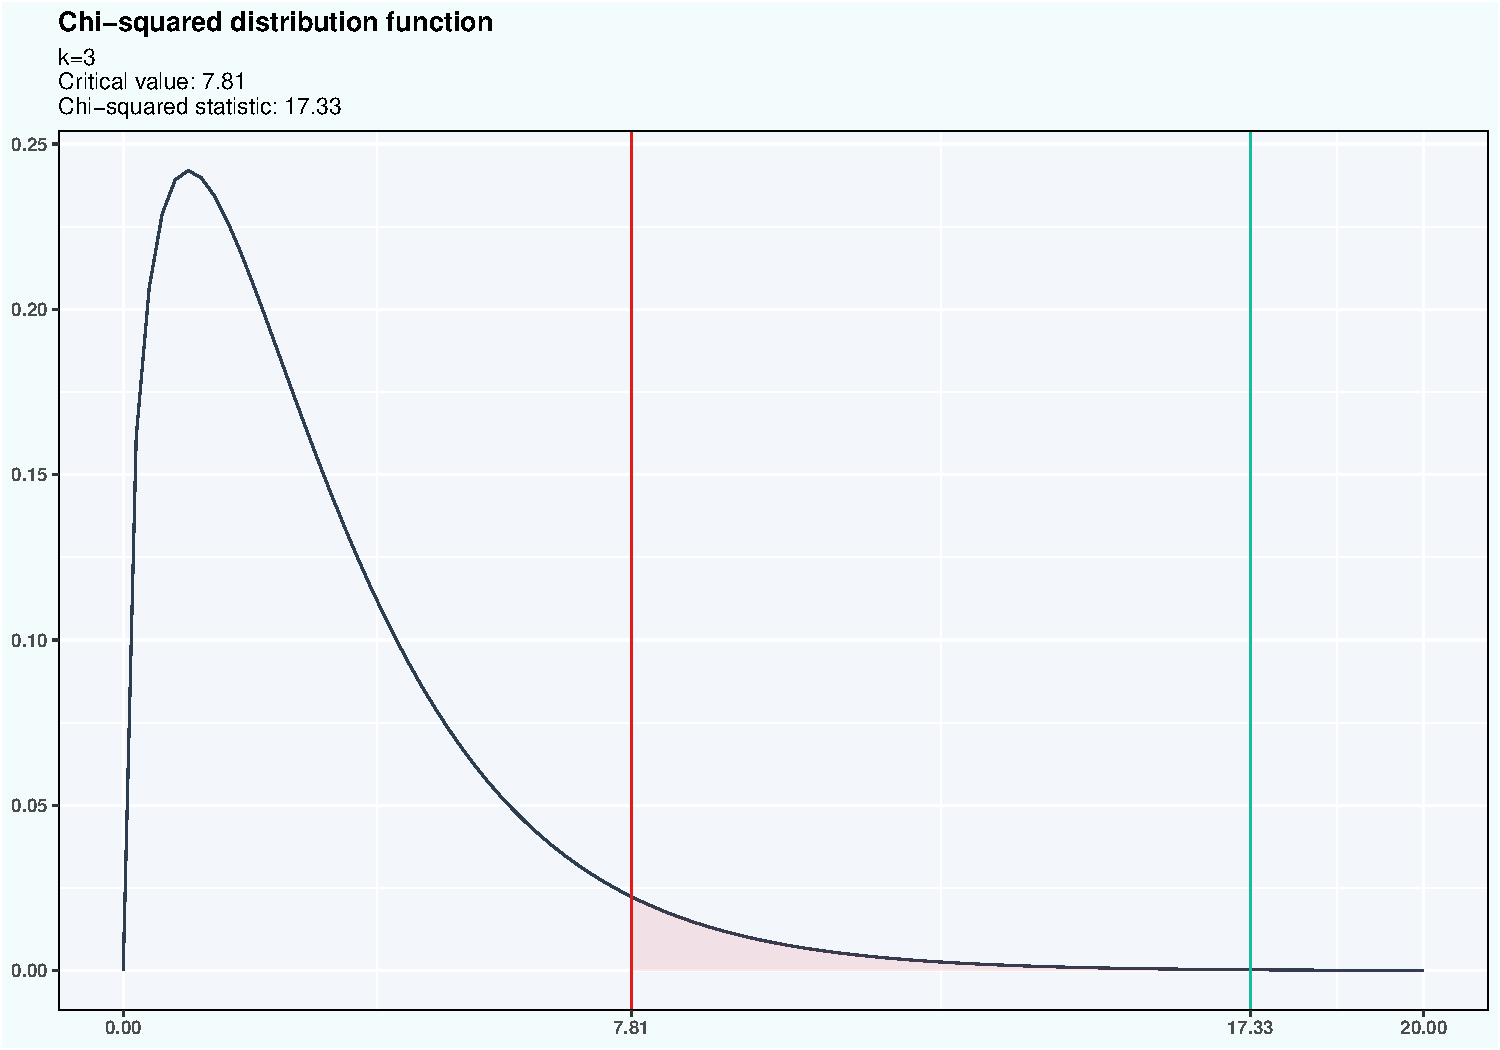
\includegraphics[width=0.85\textwidth,height=\textheight]{006_comparing_groups_statistical_tests_files/figure-beamer/unnamed-chunk-6-1.pdf}
\end{center}
\end{frame}

\begin{frame}[fragile]{}
\phantomsection\label{section-6}
\begin{itemize}
\tightlist
\item
  Chi-squared test for given probabilities
\end{itemize}

\(H_0: p_1 = \frac{1}{4} \land p_2 = \frac{1}{4} \land p_3 = \frac{1}{4} \land p_4 = \frac{1}{4}\)

\(H_1: p_1 \neq \frac{1}{4} \lor p_2 \neq \frac{1}{4} \lor p_3 = \frac{1}{4} \lor p_4 \neq \frac{1}{4}\)

\(\chi^2 = \sum_{i=1}^n \frac{(Observed_i - Expected_i)^2}{Expected_i} = \frac{70 - 300\frac{1}{4}}{300\frac{1}{4}} + \frac{100 - 300\frac{1}{4}}{300\frac{1}{4}} + \frac{80 - 300\frac{1}{4}}{300\frac{1}{4}} + \frac{50 - 300\frac{1}{4}}{300\frac{1}{4}}\)

\begin{itemize}
\tightlist
\item
  \textbf{tidymodels way}
\end{itemize}

\tiny

\begin{Shaded}
\begin{Highlighting}[]
\FunctionTok{library}\NormalTok{(tidymodels)}
\NormalTok{segmentation }\SpecialCharTok{|\textgreater{}}  
  \FunctionTok{chisq\_test}\NormalTok{(}\AttributeTok{response =}\NormalTok{ Segment,}
             \AttributeTok{p =} \FunctionTok{c}\NormalTok{(}\DecValTok{1}\SpecialCharTok{/}\DecValTok{4}\NormalTok{, }\DecValTok{1}\SpecialCharTok{/}\DecValTok{4}\NormalTok{, }\DecValTok{1}\SpecialCharTok{/}\DecValTok{4}\NormalTok{, }\DecValTok{1}\SpecialCharTok{/}\DecValTok{4}\NormalTok{))}
\end{Highlighting}
\end{Shaded}

\begin{verbatim}
# A tibble: 1 x 3
  statistic chisq_df  p_value
      <dbl>    <dbl>    <dbl>
1      17.3        3 0.000603
\end{verbatim}
\end{frame}

\begin{frame}[fragile]{}
\phantomsection\label{section-7}
\begin{itemize}
\tightlist
\item
  Pearson's Chi-squared test
\end{itemize}

\(H_0: p_{11} = \frac{260}{300}\frac{159}{300} \land p_{12} = \frac{260}{300}\frac{141}{300} \land p_{21} = \frac{40}{300}\frac{159}{300} \land p_{22} = \frac{40}{300}\frac{141}{300}\)

\(H_1: p_{11} \neq \frac{260}{300}\frac{159}{300} \lor p_{12} \neq \frac{260}{300}\frac{141}{300} \lor p_{21} \neq \frac{40}{300}\frac{159}{300} \lor p_{22} \neq \frac{40}{300}\frac{141}{300}\)

\(\chi^2 = \sum_{i=1}^n \frac{(Observed_i - Expected_i)^2}{Expected_i} = \frac{(137 - 300\frac{260}{300}\frac{159}{300})^2}{300\frac{260}{300}\frac{159}{300}} + \frac{(123 - 300\frac{260}{300}\frac{141}{300})^2}{300\frac{260}{300}\frac{141}{300}} + \frac{(22 - 300\frac{40}{300}\frac{159}{300})^2}{300\frac{40}{300}\frac{159}{300}} + \frac{(18 - 300\frac{40}{300}\frac{141}{300})^2}{300\frac{40}{300}\frac{141}{300}}\)

\begin{itemize}
\tightlist
\item
  \textbf{Base R way}
\end{itemize}

\tiny

\begin{Shaded}
\begin{Highlighting}[]
\NormalTok{chi\_statistic }\OtherTok{\textless{}{-}} \FunctionTok{chisq.test}\NormalTok{(}\FunctionTok{table}\NormalTok{(segmentation}\SpecialCharTok{$}\NormalTok{subscribe, }
\NormalTok{                 segmentation}\SpecialCharTok{$}\NormalTok{ownHome), }
           \AttributeTok{correct =} \ConstantTok{FALSE}\NormalTok{)}
\end{Highlighting}
\end{Shaded}
\end{frame}

\begin{frame}{}
\phantomsection\label{section-8}
\begin{itemize}
\tightlist
\item
  Pearson's Chi-squared test
\end{itemize}

\begin{center}
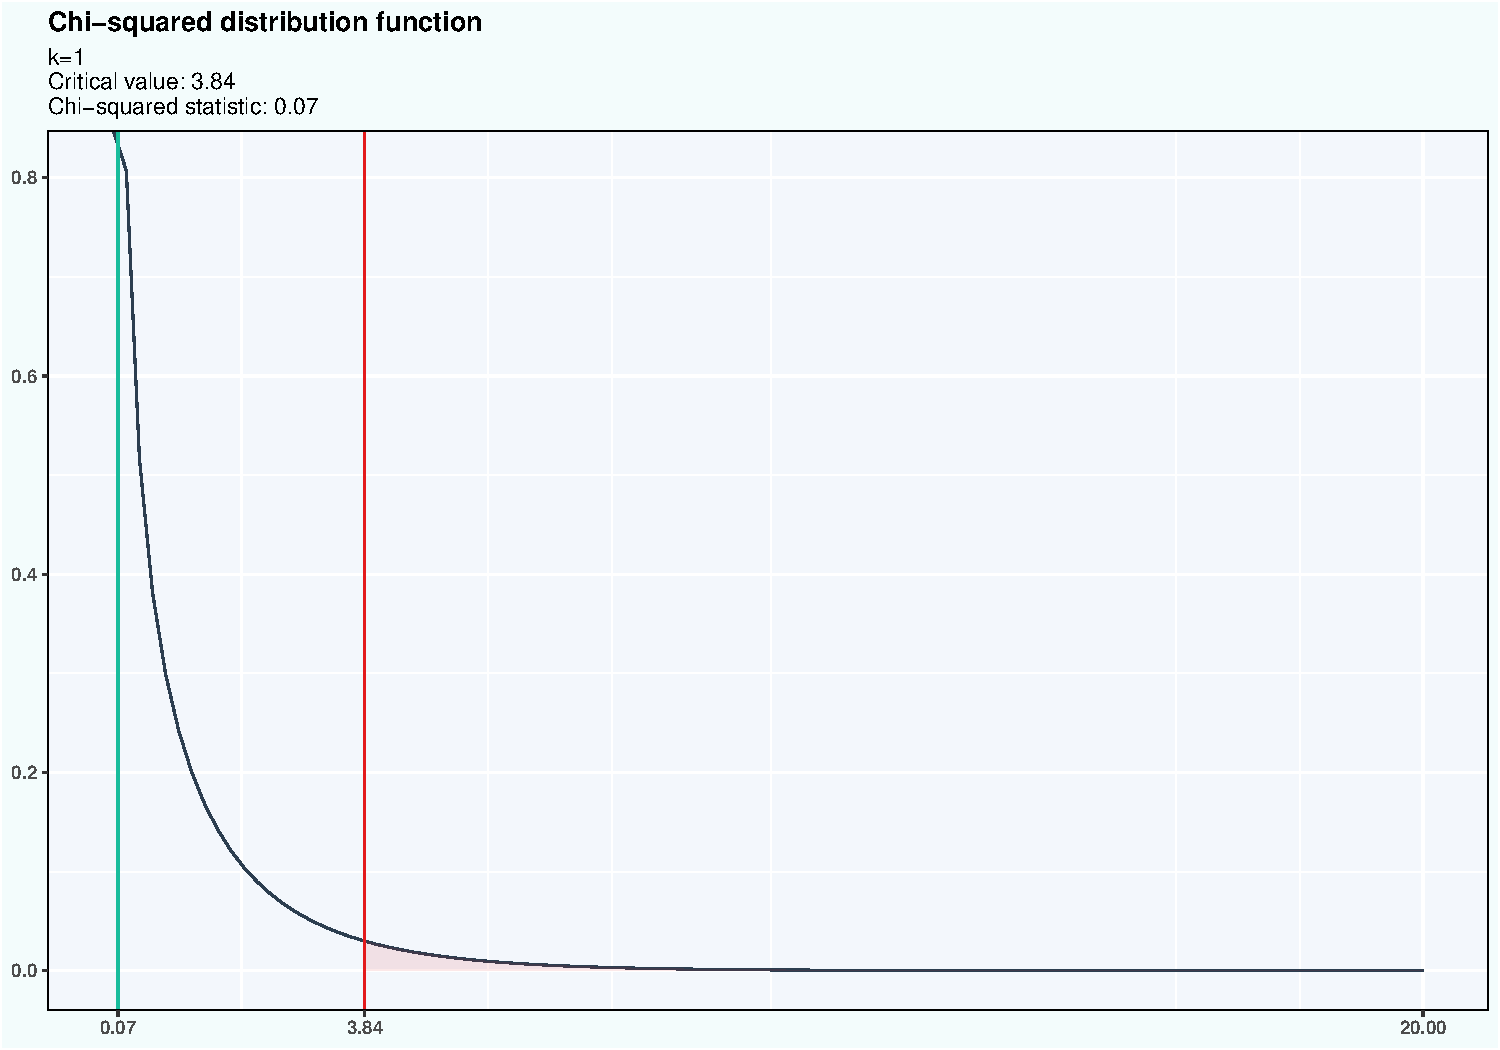
\includegraphics[width=0.85\textwidth,height=\textheight]{006_comparing_groups_statistical_tests_files/figure-beamer/unnamed-chunk-9-1.pdf}
\end{center}
\end{frame}

\begin{frame}[fragile]{}
\phantomsection\label{section-9}
\begin{itemize}
\tightlist
\item
  Pearson's Chi-squared test
\end{itemize}

\(H_0: p_{11} = \frac{260}{300}\frac{159}{300} \land p_{12} = \frac{260}{300}\frac{141}{300} \land p_{21} = \frac{40}{300}\frac{159}{300} \land p_{22} = \frac{40}{300}\frac{141}{300}\)

\(H_1: p_{11} \neq \frac{260}{300}\frac{159}{300} \lor p_{12} \neq \frac{260}{300}\frac{141}{300} \lor p_{21} \neq \frac{40}{300}\frac{159}{300} \lor p_{22} \neq \frac{40}{300}\frac{141}{300}\)

\(\chi^2 = \sum_{i=1}^n \frac{(Observed_i - Expected_i)^2}{Expected_i} = \frac{(137 - 300\frac{260}{300}\frac{159}{300})^2}{300\frac{260}{300}\frac{159}{300}} + \frac{(123 - 300\frac{260}{300}\frac{141}{300})^2}{300\frac{260}{300}\frac{141}{300}} + \frac{(22 - 300\frac{40}{300}\frac{159}{300})^2}{300\frac{40}{300}\frac{159}{300}} + \frac{(18 - 300\frac{40}{300}\frac{141}{300})^2}{300\frac{40}{300}\frac{141}{300}}\)

\begin{itemize}
\tightlist
\item
  \textbf{tidymodels way}
\end{itemize}

\tiny

\begin{Shaded}
\begin{Highlighting}[]
\NormalTok{segmentation }\SpecialCharTok{|\textgreater{}} 
  \FunctionTok{chisq\_test}\NormalTok{(}\AttributeTok{formula =}\NormalTok{ subscribe }\SpecialCharTok{\textasciitilde{}}\NormalTok{ ownHome, }
           \AttributeTok{correct =} \ConstantTok{FALSE}\NormalTok{)}
\end{Highlighting}
\end{Shaded}

\begin{verbatim}
# A tibble: 1 x 3
  statistic chisq_df p_value
      <dbl>    <int>   <dbl>
1    0.0741        1   0.785
\end{verbatim}
\end{frame}

\begin{frame}[fragile]{}
\phantomsection\label{section-10}
\begin{itemize}
\tightlist
\item
  Exact binomial test
\end{itemize}

\(H_0: p = 0.5\) \(H_1: p \neq 0.5\)

\(B = \sum_{i=1}^n x_i = 157\) where \(x_i \in {0,1}\)

\begin{itemize}
\tightlist
\item
  \textbf{R base way}
\end{itemize}

\tiny

\begin{Shaded}
\begin{Highlighting}[]
\NormalTok{binom\_test }\OtherTok{\textless{}{-}} \FunctionTok{binom.test}\NormalTok{(}\AttributeTok{x =} \DecValTok{157}\NormalTok{, }\AttributeTok{n =} \DecValTok{300}\NormalTok{, }\AttributeTok{p =} \FloatTok{0.5}\NormalTok{, }
           \AttributeTok{alternative =} \StringTok{\textquotesingle{}two.sided\textquotesingle{}}\NormalTok{,}
           \AttributeTok{conf.level =} \FloatTok{0.95}\NormalTok{)}
\NormalTok{binom\_test}
\end{Highlighting}
\end{Shaded}

\begin{verbatim}

    Exact binomial test

data:  157 and 300
number of successes = 157, number of trials = 300, p-value = 0.453
alternative hypothesis: true probability of success is not equal to 0.5
95 percent confidence interval:
 0.4651595 0.5810418
sample estimates:
probability of success 
             0.5233333 
\end{verbatim}
\end{frame}

\begin{frame}{}
\phantomsection\label{section-11}
\begin{itemize}
\tightlist
\item
  Exact binomial test
\end{itemize}

\begin{center}
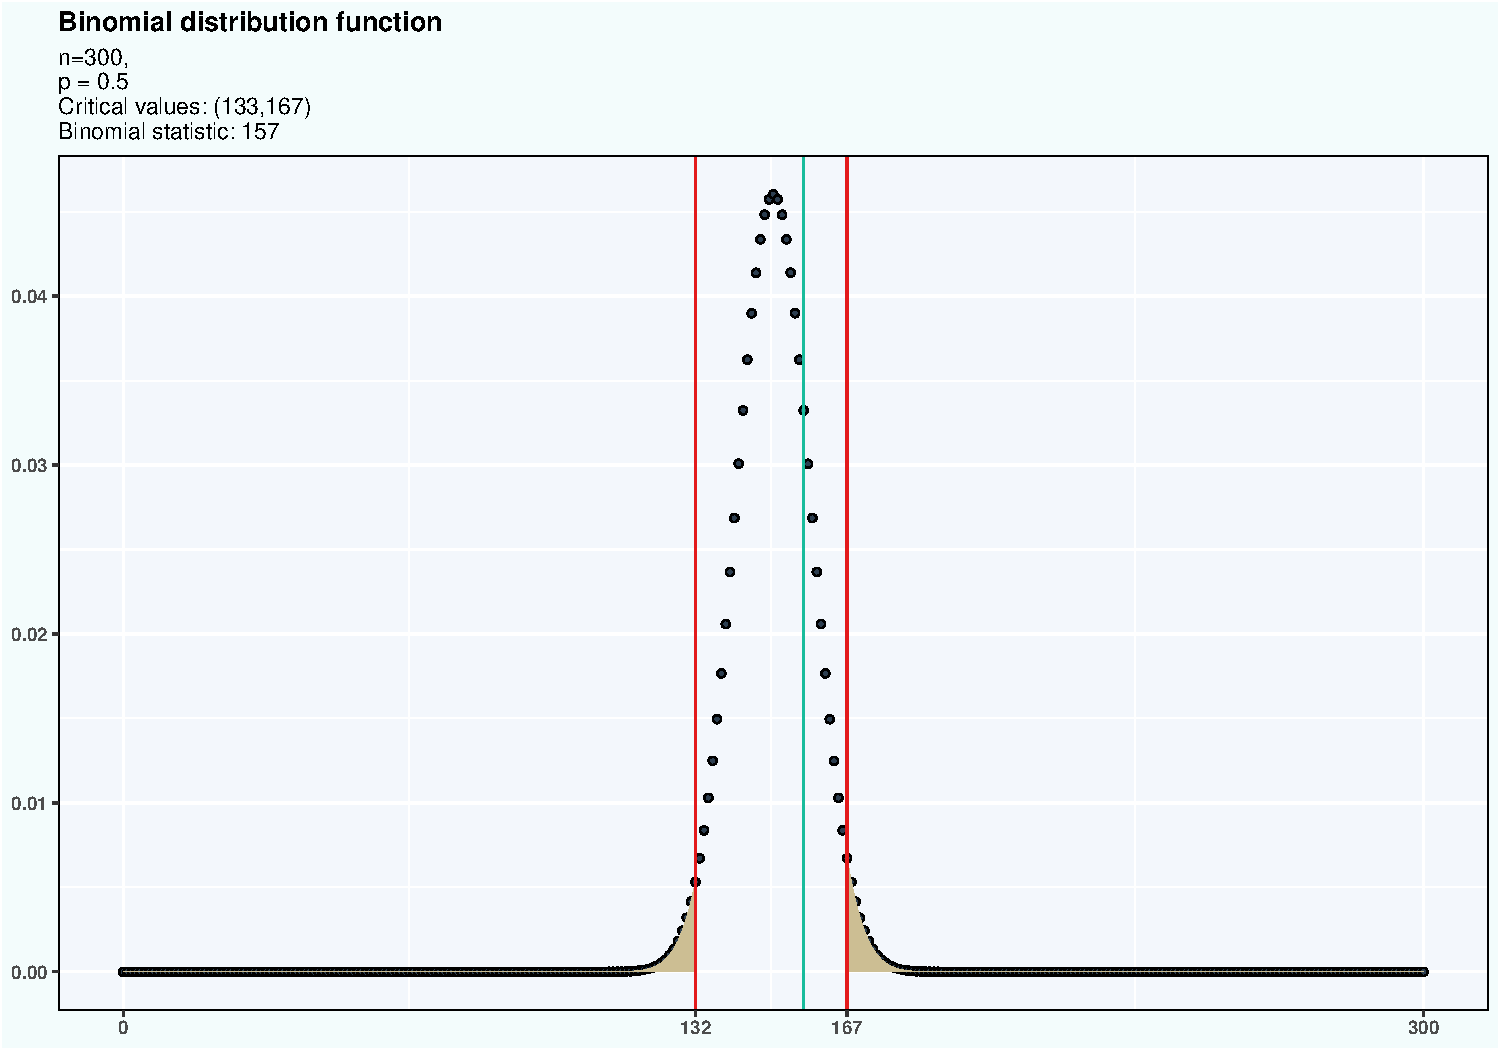
\includegraphics[width=0.85\textwidth,height=\textheight]{006_comparing_groups_statistical_tests_files/figure-beamer/unnamed-chunk-12-1.pdf}
\end{center}
\end{frame}

\begin{frame}{}
\phantomsection\label{section-12}
\begin{itemize}
\item
  Exact binomial test

  \begin{itemize}
  \tightlist
  \item
    Confidence interval:
  \end{itemize}
\end{itemize}

\[p_L < p < p_U\]

\begin{itemize}
\tightlist
\item
  \(p_L\) and \(p_U\) are random variables but \(p\) is not a random
  variable. Therefore \([p_L, p_U]\) is a random interval where we have
  that:
\end{itemize}

\[P(0.4651595 \approx p_L < p < p_U \approx 0.5810418) = 0.95\]
\end{frame}

\begin{frame}[fragile]{}
\phantomsection\label{section-13}
\begin{itemize}
\tightlist
\item
  Exact binomial test
\end{itemize}

\(H_0: p = 0.5\) \(H_1: p \neq 0.5\)

\(B = \sum_{i=1}^n x_i = 157\) where \(x_i \in {0,1}\)

\begin{itemize}
\tightlist
\item
  \textbf{tidymodels way}
\end{itemize}

\tiny

\begin{Shaded}
\begin{Highlighting}[]
\FunctionTok{binom.test}\NormalTok{(}\AttributeTok{x =} \DecValTok{157}\NormalTok{, }\AttributeTok{n =} \DecValTok{300}\NormalTok{, }\AttributeTok{p =} \FloatTok{0.5}\NormalTok{, }
           \AttributeTok{alternative =} \StringTok{\textquotesingle{}two.sided\textquotesingle{}}\NormalTok{,}
           \AttributeTok{conf.level =} \FloatTok{0.95}\NormalTok{) }\SpecialCharTok{|\textgreater{}} 
  \FunctionTok{tidy}\NormalTok{()}
\end{Highlighting}
\end{Shaded}

\begin{verbatim}
# A tibble: 1 x 8
  estimate statistic p.value parameter conf.low conf.high method     alternative
     <dbl>     <dbl>   <dbl>     <dbl>    <dbl>     <dbl> <chr>      <chr>      
1    0.523       157   0.453       300    0.465     0.581 Exact bin~ two.sided  
\end{verbatim}
\end{frame}

\begin{frame}[fragile]{}
\phantomsection\label{section-14}
\begin{itemize}
\tightlist
\item
  2 sample t-test: independent samples
\end{itemize}

\tiny

\begin{Shaded}
\begin{Highlighting}[]
\NormalTok{segmentation }\SpecialCharTok{|\textgreater{}} \FunctionTok{ggplot}\NormalTok{() }\SpecialCharTok{+} 
  \FunctionTok{geom\_histogram}\NormalTok{(}\FunctionTok{aes}\NormalTok{(}\AttributeTok{x =}\NormalTok{ income), }\AttributeTok{color=}\StringTok{\textquotesingle{}black\textquotesingle{}}\NormalTok{) }\SpecialCharTok{+} 
  \FunctionTok{facet\_wrap}\NormalTok{(}\AttributeTok{facets =} \FunctionTok{vars}\NormalTok{(ownHome))}
\end{Highlighting}
\end{Shaded}

\begin{center}
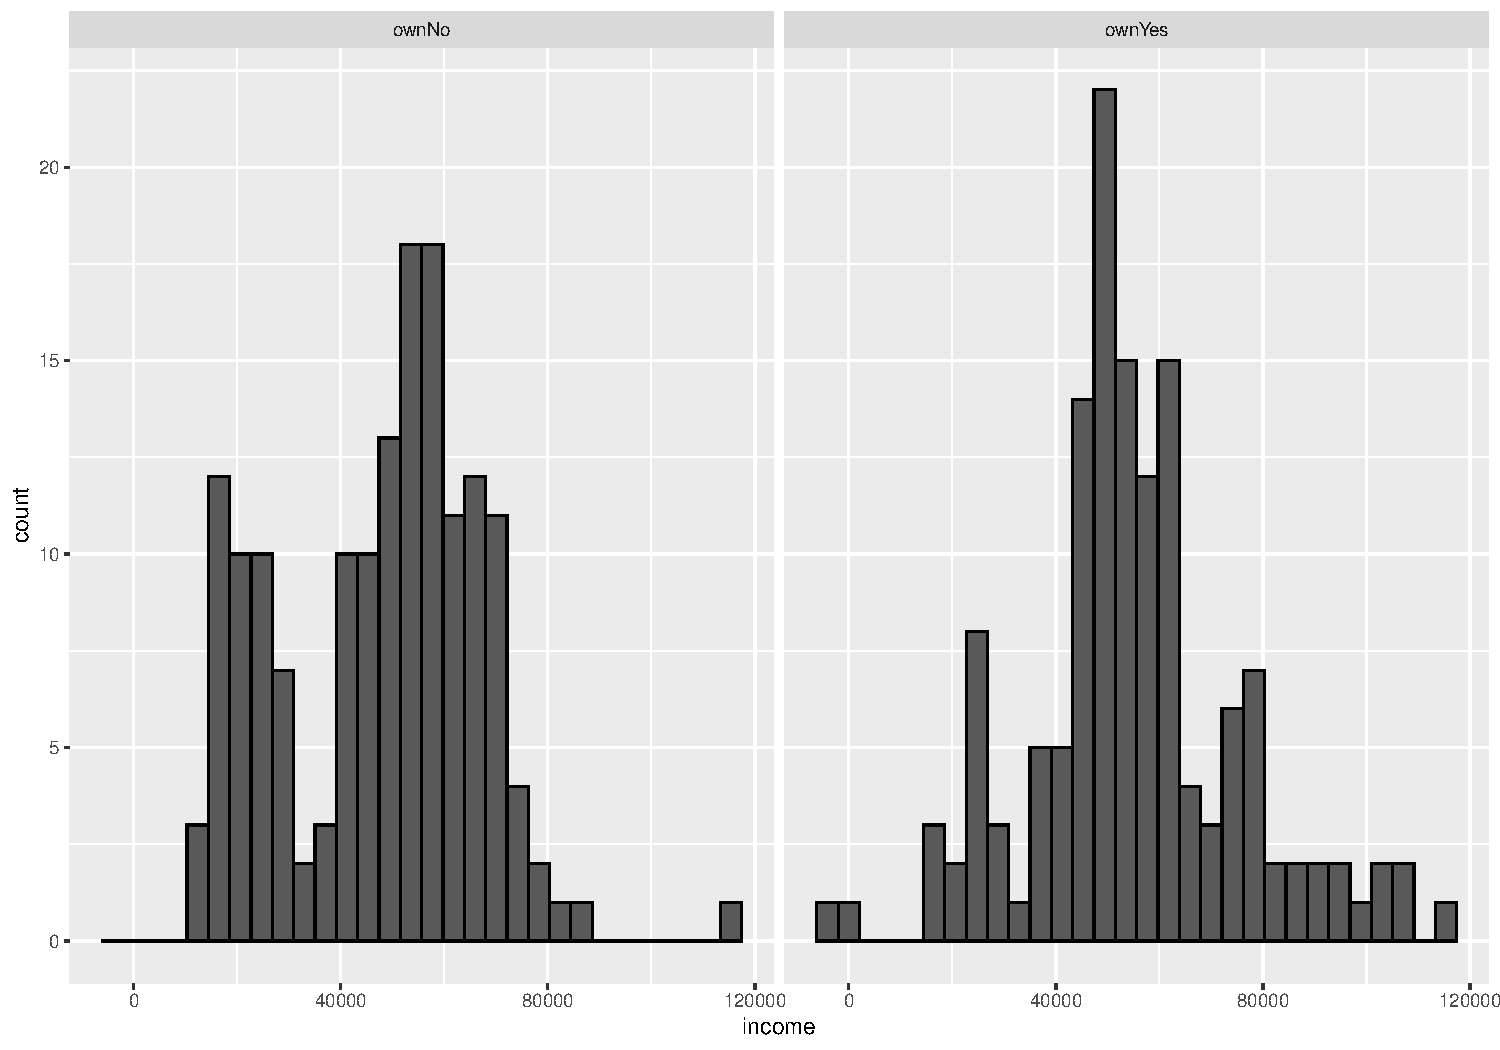
\includegraphics[width=0.85\textwidth,height=\textheight]{006_comparing_groups_statistical_tests_files/figure-beamer/unnamed-chunk-14-1.pdf}
\end{center}
\end{frame}

\begin{frame}[fragile]{}
\phantomsection\label{section-15}
\begin{itemize}
\tightlist
\item
  2 sample t-test: independent samples
\end{itemize}

\tiny

\begin{Shaded}
\begin{Highlighting}[]
\NormalTok{segmentation }\SpecialCharTok{|\textgreater{}} 
  \FunctionTok{group\_by}\NormalTok{(ownHome) }\SpecialCharTok{|\textgreater{}} 
  \FunctionTok{summarise}\NormalTok{(}\AttributeTok{mean\_income =} \FunctionTok{mean}\NormalTok{(income),}
            \AttributeTok{var\_income =} \FunctionTok{var}\NormalTok{(income),}
            \AttributeTok{n =} \FunctionTok{n}\NormalTok{())}
\end{Highlighting}
\end{Shaded}

\begin{verbatim}
# A tibble: 2 x 4
  ownHome mean_income var_income     n
  <chr>         <dbl>      <dbl> <int>
1 ownNo        47391. 358692875.   159
2 ownYes       54935. 430890091.   141
\end{verbatim}
\end{frame}

\begin{frame}[fragile]{}
\phantomsection\label{section-16}
\begin{itemize}
\tightlist
\item
  2 sample t-test: independent samples
\end{itemize}

\(H_0: \mu_{ownNo} - \mu_{ownYes}= 0\)
\(H_1: \mu_{ownNo} - \mu_{ownYes} \neq 0\)

\(t = \frac{\overline{ownNo} - \overline{ownYes}}{\sqrt{\frac{s_{ownNo}^2}{n_{ownNo}} - \frac{s_{ownYes}^2}{n_{ownYes}}}} = \frac{47391.01 - 54934.68}{\sqrt{ \frac{358692875}{159} - \frac{430890091}{141}}} \approx -3.273094\)

\begin{itemize}
\tightlist
\item
  \textbf{R base way}
\end{itemize}

\tiny

\begin{Shaded}
\begin{Highlighting}[]
\NormalTok{t\_test }\OtherTok{\textless{}{-}} \FunctionTok{t.test}\NormalTok{(income }\SpecialCharTok{\textasciitilde{}}\NormalTok{ ownHome, }\AttributeTok{data =}\NormalTok{ segmentation,}
                 \AttributeTok{alternative=}\StringTok{\textquotesingle{}two.sided\textquotesingle{}}\NormalTok{, }\AttributeTok{mu =} \DecValTok{0}\NormalTok{,}
                 \AttributeTok{conf.level =} \FloatTok{0.95}\NormalTok{)}
\NormalTok{t\_test}
\end{Highlighting}
\end{Shaded}

\begin{verbatim}

    Welch Two Sample t-test

data:  income by ownHome
t = -3.2731, df = 285.25, p-value = 0.001195
alternative hypothesis: true difference in means between group ownNo and group ownYes is not equal to 0
95 percent confidence interval:
 -12080.155  -3007.193
sample estimates:
 mean in group ownNo mean in group ownYes 
            47391.01             54934.68 
\end{verbatim}
\end{frame}

\begin{frame}{}
\phantomsection\label{section-17}
\begin{itemize}
\tightlist
\item
  2 sample t-test: independent samples
\end{itemize}

\begin{center}
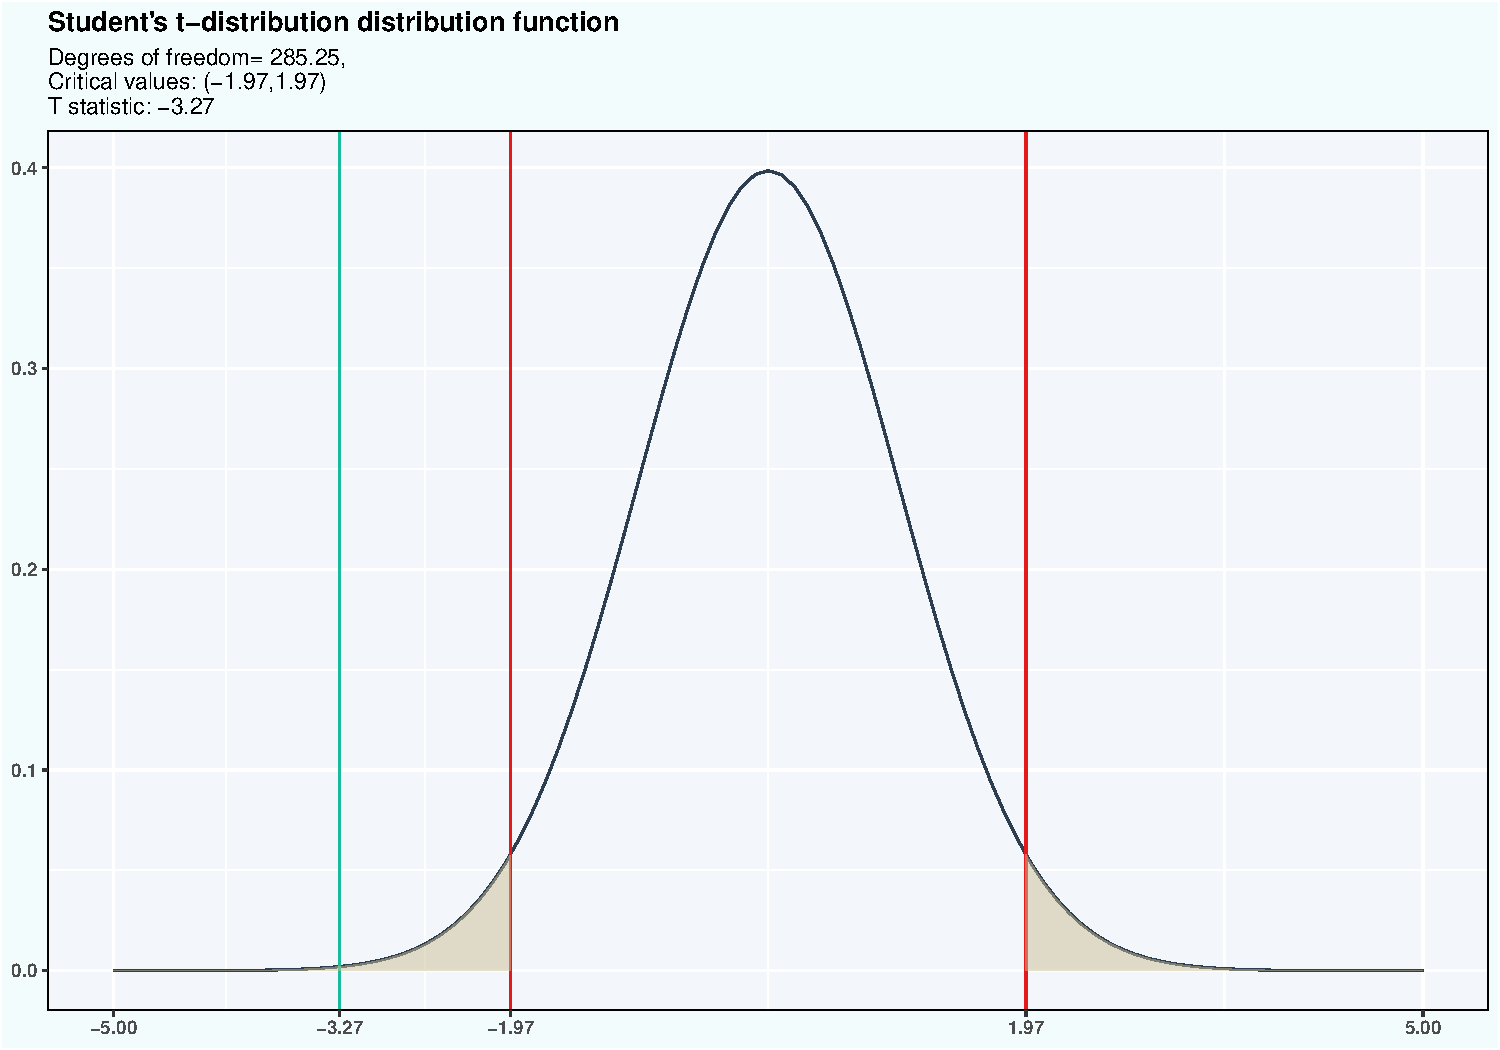
\includegraphics[width=0.85\textwidth,height=\textheight]{006_comparing_groups_statistical_tests_files/figure-beamer/unnamed-chunk-17-1.pdf}
\end{center}
\end{frame}

\begin{frame}{}
\phantomsection\label{section-18}
\begin{itemize}
\item
  2 sample t-test: independent samples

  \begin{itemize}
  \tightlist
  \item
    Confidence interval:
  \end{itemize}
\end{itemize}

\[c_L < \mu_{ownNo} - \mu_{ownYes} < c_U\]

\begin{itemize}
\tightlist
\item
  \(\mu_{ownNo} - \mu_{ownYes}\) is not a random variable so we need to
  use a random variable
\end{itemize}

\[P \Biggr( t_L < \frac{\overline{x}_{ownNo} - \overline{x}_{ownYes} - (\mu_{ownNo} - \mu_{ownYes})}{\sqrt{\frac{s^2_{ownNo}}{n_{ownNo} } +\frac{s^2_{ownYes}}{n_{ownYes}}}} < t_U \Biggr) = 0.95\]

\begin{itemize}
\tightlist
\item
  \(\overline{x}_{ownNo} - \overline{x}_{ownYes}\) is a random variable
\end{itemize}
\end{frame}

\begin{frame}[fragile]{}
\phantomsection\label{section-19}
\begin{itemize}
\item
  2 sample t-test: independent samples

  \begin{itemize}
  \item
    Confidence interval:

    \begin{itemize}
    \item
      \(\frac{\overline{x}_{ownNo} - \overline{x}_{ownYes} - (\mu_{ownNo} - \mu_{ownYes})}{\sqrt{\frac{s^2_{ownNo}}{n_{ownNo} } +\frac{s^2_{ownYes}}{n_{ownYes}}}}\)
      is also a random variable with student's t-distribution and
      \(\nu \approx \frac{(\frac{s_{ownNo}^2}{n_{ownNo}} + \frac{s_2^2}{n_{ownYes}})^2}{\frac{(\frac{s_{ownNo}^2}{n_{ownNo}})^2}{n_{ownNo}-1} + \frac{(\frac{s_2^2}{n_{ownYes}})^2}{n_{ownYes}-1}} = 285.2521\)
      degrees of freedom
    \item
      Also we need to specify \(t_L\) and \(t_U\)
    \end{itemize}
  \end{itemize}
\end{itemize}

\tiny

\begin{Shaded}
\begin{Highlighting}[]
\NormalTok{t\_L }\OtherTok{\textless{}{-}} \FunctionTok{qt}\NormalTok{(}\AttributeTok{p =} \FloatTok{0.025}\NormalTok{, }\AttributeTok{df =} \FloatTok{285.25}\NormalTok{, }\AttributeTok{lower.tail =} \ConstantTok{TRUE}\NormalTok{)}
\NormalTok{t\_L}
\end{Highlighting}
\end{Shaded}

\begin{verbatim}
[1] -1.968315
\end{verbatim}

\begin{Shaded}
\begin{Highlighting}[]
\NormalTok{t\_U }\OtherTok{\textless{}{-}} \FunctionTok{qt}\NormalTok{(}\AttributeTok{p =} \FloatTok{0.975}\NormalTok{, }\AttributeTok{df =} \FloatTok{285.25}\NormalTok{, }\AttributeTok{lower.tail =} \ConstantTok{TRUE}\NormalTok{)}
\NormalTok{t\_U}
\end{Highlighting}
\end{Shaded}

\begin{verbatim}
[1] 1.968315
\end{verbatim}
\end{frame}

\begin{frame}{}
\phantomsection\label{section-20}
\begin{itemize}
\item
  2 sample t-test: independent samples

  \begin{itemize}
  \tightlist
  \item
    Confidence interval:
  \end{itemize}
\end{itemize}

\tiny

\[P(-7543.674 - 1.968315\times2304.753 < \mu_{ownNo} - \mu_{ownYes} < -7543.674 - 1.968315\times2304.753) = 0.95\]
\[P(-12080.16 < \mu_{ownNo} - \mu_{ownYes} < -3007.193) = 0.95\]

\normalsize

\begin{itemize}
\tightlist
\item
  In the long run 95\% of confidence intervals constructed in this
  manner will contain the true parameter
\end{itemize}
\end{frame}

\begin{frame}[fragile]{}
\phantomsection\label{section-21}
\begin{itemize}
\tightlist
\item
  2 sample t-test: independent samples
\end{itemize}

\(H_0: \mu_{ownNo} - \mu_{ownYes}= 0\)
\(H_1: \mu_{ownNo} - \mu_{ownYes} \neq 0\)

\(t = \frac{\overline{ownNo} - \overline{ownYes}}{\sqrt{\frac{s_{ownNo}^2}{n_{ownNo}} - \frac{s_{ownYes}^2}{n_{ownYes}}}} = \frac{47391.01 - 54934.68}{\sqrt{ \frac{358692875}{159} - \frac{430890091}{141}}} \approx -3.273094\)

\begin{itemize}
\tightlist
\item
  \textbf{tidymodels way}
\end{itemize}

\tiny

\begin{Shaded}
\begin{Highlighting}[]
\NormalTok{segmentation }\SpecialCharTok{|\textgreater{}} 
  \FunctionTok{t\_test}\NormalTok{(}\AttributeTok{formula =}\NormalTok{ income }\SpecialCharTok{\textasciitilde{}}\NormalTok{ ownHome,}
         \AttributeTok{alternative =} \StringTok{"two{-}sided"}\NormalTok{,}
         \AttributeTok{order =} \FunctionTok{c}\NormalTok{(}\StringTok{"ownNo"}\NormalTok{, }\StringTok{"ownYes"}\NormalTok{),}
         \AttributeTok{mu =} \DecValTok{0}\NormalTok{,}
         \AttributeTok{conf\_level =} \FloatTok{0.95}\NormalTok{)}
\end{Highlighting}
\end{Shaded}

\begin{verbatim}
# A tibble: 1 x 7
  statistic  t_df p_value alternative estimate lower_ci upper_ci
      <dbl> <dbl>   <dbl> <chr>          <dbl>    <dbl>    <dbl>
1     -3.27  285. 0.00119 two.sided     -7544.  -12080.   -3007.
\end{verbatim}
\end{frame}

\begin{frame}[fragile]{}
\phantomsection\label{section-22}
\begin{itemize}
\tightlist
\item
  Testing Multiple Group Means: Analysis of Variance (ANOVA)
\end{itemize}

\tiny

\begin{Shaded}
\begin{Highlighting}[]
\NormalTok{segmentation }\SpecialCharTok{|\textgreater{}} 
  \FunctionTok{group\_by}\NormalTok{(Segment) }\SpecialCharTok{|\textgreater{}} 
  \FunctionTok{summarise}\NormalTok{(}\AttributeTok{mean =} \FunctionTok{mean}\NormalTok{(income),}
            \AttributeTok{variance =} \FunctionTok{var}\NormalTok{(income),}
            \AttributeTok{n =} \FunctionTok{n}\NormalTok{())}
\end{Highlighting}
\end{Shaded}

\begin{verbatim}
# A tibble: 4 x 4
  Segment      mean   variance     n
  <chr>       <dbl>      <dbl> <int>
1 Moving up  53091.  92862689.    70
2 Suburb mix 55034. 142761527.   100
3 Travelers  62214. 564173979.    80
4 Urban hip  21682.  23885953.    50
\end{verbatim}
\end{frame}

\begin{frame}{}
\phantomsection\label{section-23}
\begin{itemize}
\tightlist
\item
  Testing Multiple Group Means: Analysis of Variance (ANOVA)
\end{itemize}

\begin{center}
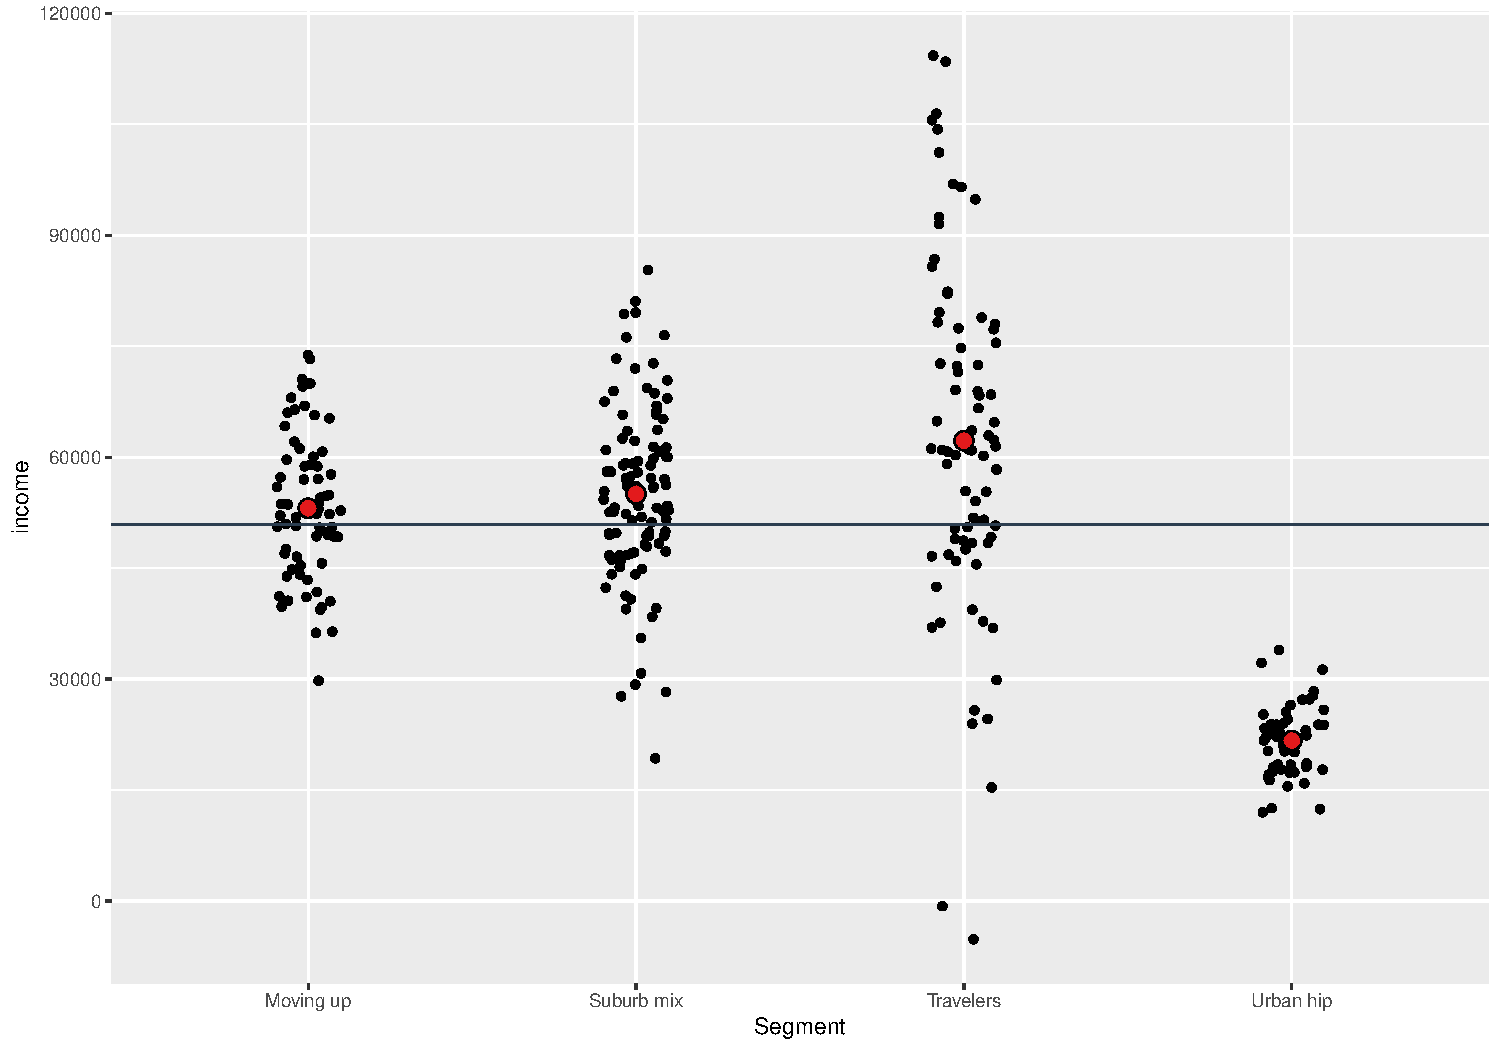
\includegraphics[width=0.85\textwidth,height=\textheight]{006_comparing_groups_statistical_tests_files/figure-beamer/unnamed-chunk-21-1.pdf}
\end{center}
\end{frame}

\begin{frame}{}
\phantomsection\label{section-24}
\begin{itemize}
\tightlist
\item
  Testing Multiple Group Means: Analysis of Variance (ANOVA)
\end{itemize}

\(H_0: \mu_{Moving\;up} = \mu_{Suburb\;mix} = \mu_{Travelers} = \mu_{Urban\;hip}\)

\(H_1: \text{At least one group mean is different from the rest}\)

\(n = \sum_{j=1}^4 n_j = n_1 + \cdots + n_4 = 70 + 100 + 80 + 50 = 300\)

\(\overline{income} = \frac{1}{n} \sum_{j=1}^4 \sum_{i=1}^{n_j} income_{ij}\)

\(\overline{income}_j = \frac{1}{n_j} \sum_{i=1}^{n_j} income_{ij}\)

\(F = \frac{\frac{\sum_{j=1}^4 \sum_{i=1}^{n_j} (\overline{income}_j - \overline{income})^2}{4-1}}{\frac{\sum_{j=1}^4 \sum_{i=1}^{n_j} (income_{ij} - \overline{income}_j)^2}{300 - 4}} = \frac{\frac{54969675428}{3}}{\frac{66281072794}{296}} = \frac{18323225143}{223922543} = 81.82841\)
\end{frame}

\begin{frame}[fragile]{}
\phantomsection\label{section-25}
\begin{itemize}
\item
  Testing Multiple Group Means: Analysis of Variance (ANOVA)

  \begin{itemize}
  \tightlist
  \item
    \textbf{R base way}
  \end{itemize}
\end{itemize}

\tiny

\begin{Shaded}
\begin{Highlighting}[]
\NormalTok{anova\_table }\OtherTok{\textless{}{-}} \FunctionTok{aov}\NormalTok{(}\AttributeTok{data =}\NormalTok{ segmentation, }\AttributeTok{formula =}\NormalTok{ income }\SpecialCharTok{\textasciitilde{}}\NormalTok{ Segment) }\SpecialCharTok{|\textgreater{}}
  \FunctionTok{anova}\NormalTok{()}
\NormalTok{anova\_table}
\end{Highlighting}
\end{Shaded}

\begin{verbatim}
Analysis of Variance Table

Response: income
           Df     Sum Sq    Mean Sq F value    Pr(>F)    
Segment     3 5.4970e+10 1.8323e+10  81.828 < 2.2e-16 ***
Residuals 296 6.6281e+10 2.2392e+08                      
---
Signif. codes:  0 '***' 0.001 '**' 0.01 '*' 0.05 '.' 0.1 ' ' 1
\end{verbatim}
\end{frame}

\begin{frame}{}
\phantomsection\label{section-26}
\begin{itemize}
\tightlist
\item
  Testing Multiple Group Means: Analysis of Variance (ANOVA)
\end{itemize}

\begin{center}
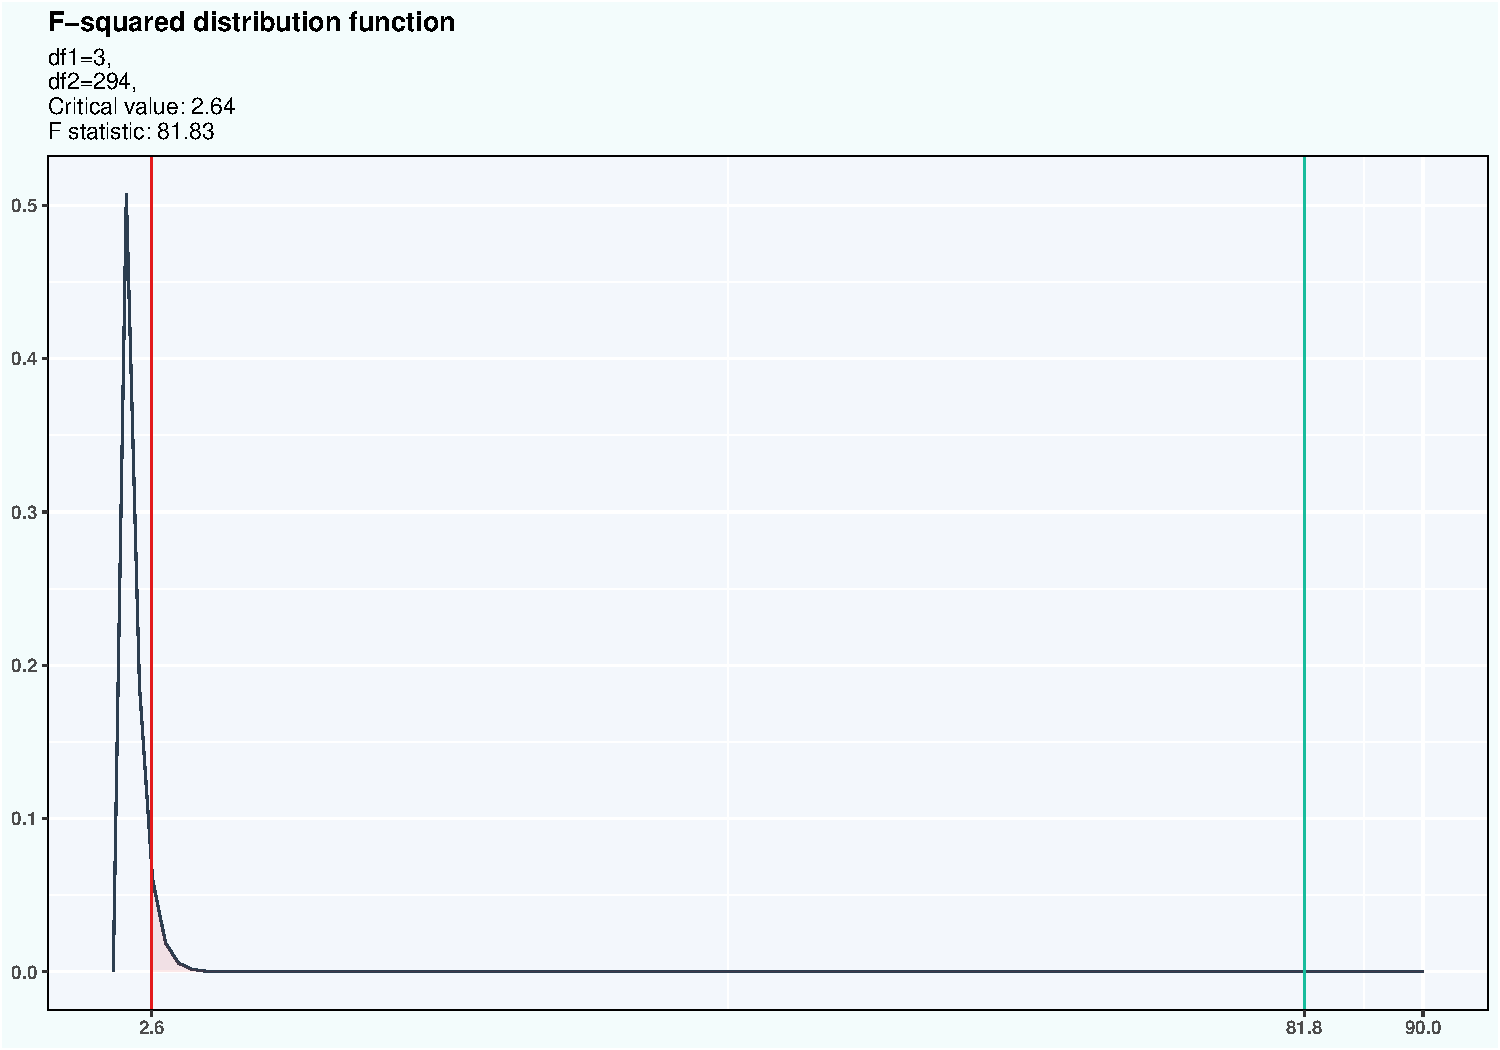
\includegraphics[width=0.85\textwidth,height=\textheight]{006_comparing_groups_statistical_tests_files/figure-beamer/unnamed-chunk-23-1.pdf}
\end{center}
\end{frame}

\begin{frame}[fragile]{}
\phantomsection\label{section-27}
\begin{itemize}
\item
  Testing Multiple Group Means: Analysis of Variance (ANOVA)

  \begin{itemize}
  \tightlist
  \item
    \textbf{tidymodels way}
  \end{itemize}
\end{itemize}

\tiny

\begin{Shaded}
\begin{Highlighting}[]
\NormalTok{anova\_table }\OtherTok{\textless{}{-}} \FunctionTok{aov}\NormalTok{(}\AttributeTok{data =}\NormalTok{ segmentation, }\AttributeTok{formula =}\NormalTok{ income }\SpecialCharTok{\textasciitilde{}}\NormalTok{ Segment) }\SpecialCharTok{|\textgreater{}}
  \FunctionTok{anova}\NormalTok{() }\SpecialCharTok{|\textgreater{}} 
  \FunctionTok{tidy}\NormalTok{()}
\NormalTok{anova\_table}
\end{Highlighting}
\end{Shaded}

\begin{verbatim}
# A tibble: 2 x 6
  term         df        sumsq       meansq statistic   p.value
  <chr>     <int>        <dbl>        <dbl>     <dbl>     <dbl>
1 Segment       3 54969675428. 18323225143.      81.8  1.41e-38
2 Residuals   296 66281072794.   223922543.      NA   NA       
\end{verbatim}
\end{frame}

\begin{frame}[fragile]{}
\phantomsection\label{section-28}
\begin{itemize}
\tightlist
\item
  Testing Multiple Group Means: Analysis of Variance (ANOVA)
\end{itemize}

\tiny

\begin{Shaded}
\begin{Highlighting}[]
\NormalTok{segmentation }\SpecialCharTok{|\textgreater{}} 
  \FunctionTok{distinct}\NormalTok{(Segment) }\SpecialCharTok{|\textgreater{}} 
  \FunctionTok{arrange}\NormalTok{(Segment) }\SpecialCharTok{|\textgreater{}} 
  \FunctionTok{rowid\_to\_column}\NormalTok{(}\AttributeTok{var =} \StringTok{\textquotesingle{}i\textquotesingle{}}\NormalTok{)}
\end{Highlighting}
\end{Shaded}

\begin{verbatim}
# A tibble: 4 x 2
      i Segment   
  <int> <chr>     
1     1 Moving up 
2     2 Suburb mix
3     3 Travelers 
4     4 Urban hip 
\end{verbatim}

\tiny

\begin{Shaded}
\begin{Highlighting}[]
\NormalTok{segmentation }\SpecialCharTok{|\textgreater{}} 
  \FunctionTok{distinct}\NormalTok{(ownHome) }\SpecialCharTok{|\textgreater{}} 
  \FunctionTok{rowid\_to\_column}\NormalTok{(}\AttributeTok{var =} \StringTok{\textquotesingle{}j\textquotesingle{}}\NormalTok{)}
\end{Highlighting}
\end{Shaded}

\begin{verbatim}
# A tibble: 2 x 2
      j ownHome
  <int> <chr>  
1     1 ownNo  
2     2 ownYes 
\end{verbatim}
\end{frame}

\begin{frame}[fragile]{}
\phantomsection\label{section-29}
\begin{itemize}
\tightlist
\item
  Testing Multiple Group Means: Analysis of Variance (ANOVA)
\end{itemize}

\tiny

\begin{Shaded}
\begin{Highlighting}[]
\NormalTok{segmentation }\SpecialCharTok{|\textgreater{}} 
  \FunctionTok{count}\NormalTok{(Segment, ownHome, }\AttributeTok{name =} \StringTok{"n\_ij"}\NormalTok{)}
\end{Highlighting}
\end{Shaded}

\begin{verbatim}
# A tibble: 8 x 3
  Segment    ownHome  n_ij
  <chr>      <chr>   <int>
1 Moving up  ownNo      47
2 Moving up  ownYes     23
3 Suburb mix ownNo      52
4 Suburb mix ownYes     48
5 Travelers  ownNo      20
6 Travelers  ownYes     60
7 Urban hip  ownNo      40
8 Urban hip  ownYes     10
\end{verbatim}
\end{frame}

\begin{frame}[fragile]{}
\phantomsection\label{section-30}
\begin{itemize}
\tightlist
\item
  Testing Multiple Group Means: Analysis of Variance (ANOVA)
\end{itemize}

\tiny

\begin{Shaded}
\begin{Highlighting}[]
\NormalTok{mu\_ij }\OtherTok{\textless{}{-}}\NormalTok{ segmentation }\SpecialCharTok{|\textgreater{}} 
  \FunctionTok{group\_by}\NormalTok{(Segment, ownHome) }\SpecialCharTok{|\textgreater{}} 
  \FunctionTok{summarise}\NormalTok{(}\AttributeTok{mean =} \FunctionTok{mean}\NormalTok{(income)) }\SpecialCharTok{|\textgreater{}} 
  \FunctionTok{ungroup}\NormalTok{()}
\NormalTok{mu\_11 }\OtherTok{\textless{}{-}}\NormalTok{ mu\_ij}\SpecialCharTok{$}\NormalTok{mean[}\DecValTok{1}\NormalTok{]}
\NormalTok{mu\_11}
\end{Highlighting}
\end{Shaded}

\begin{verbatim}
[1] 54497.68
\end{verbatim}

\begin{Shaded}
\begin{Highlighting}[]
\NormalTok{segmentation }\SpecialCharTok{|\textgreater{}} 
  \FunctionTok{select}\NormalTok{(income, Segment, ownHome) }\SpecialCharTok{|\textgreater{}} 
  \FunctionTok{head}\NormalTok{(}\AttributeTok{n=}\DecValTok{5}\NormalTok{)}
\end{Highlighting}
\end{Shaded}

\begin{verbatim}
# A tibble: 5 x 3
  income Segment    ownHome
   <dbl> <chr>      <chr>  
1 49483. Suburb mix ownNo  
2 35546. Suburb mix ownYes 
3 44169. Suburb mix ownYes 
4 81042. Suburb mix ownNo  
5 79353. Suburb mix ownYes 
\end{verbatim}
\end{frame}

\begin{frame}{}
\phantomsection\label{section-31}
\begin{itemize}
\tightlist
\item
  Testing Multiple Group Means: Analysis of Variance (ANOVA)
\end{itemize}

\begin{center}
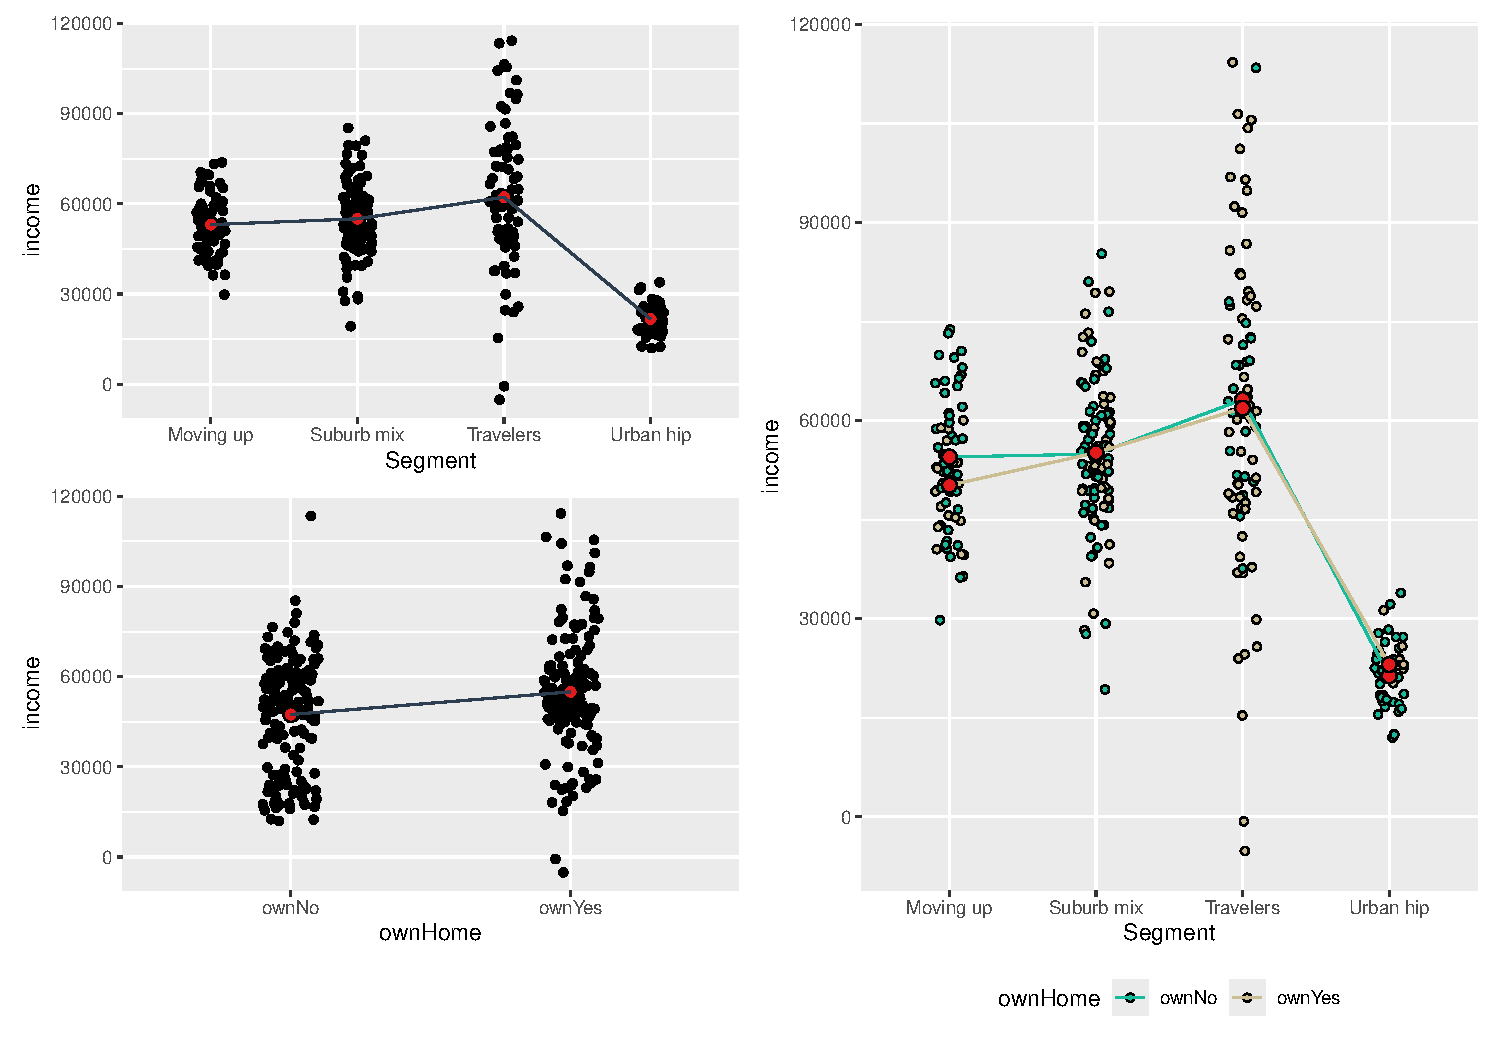
\includegraphics[width=0.85\textwidth,height=\textheight]{006_comparing_groups_statistical_tests_files/figure-beamer/unnamed-chunk-30-1.pdf}
\end{center}
\end{frame}

\begin{frame}{}
\phantomsection\label{section-32}
\begin{itemize}
\tightlist
\item
  Testing Multiple Group Means: Analysis of Variance (ANOVA)
\end{itemize}

\footnotesize

\[\begin{split}
  income_{ijk} =  & \mu + \alpha_i + \beta_j + (\alpha\beta)_{ij} + \epsilon_{ijk} \\ 
  & \text{ where } + \epsilon_i \sim \mathcal{N}(0, \sigma^2) \\ 
  & \text{ and } i = 1, 2, 3, 4 \\
  & j = 1, 2 \\
  & k = 1, \ldots n_{ij} \\
  & \mu = \mu_{11} \\
  & \alpha_1 = \beta_1 = 0 \\
  & (\alpha\beta)_{11} = (\alpha\beta)_{12} = 0 \\ 
  & (\alpha\beta)_{21} = (\alpha\beta)_{31} = (\alpha\beta)_{41} = 0 \\  
  \end{split}\]
\end{frame}

\begin{frame}{}
\phantomsection\label{section-33}
\begin{itemize}
\tightlist
\item
  Testing Multiple Group Means: Analysis of Variance (ANOVA)
\end{itemize}

\footnotesize

\[\begin{split}
  \widehat{income}_{ijk} =  & \widehat{\mu} + \widehat{\alpha}_i + \widehat{\beta}_j + (\widehat{\alpha\beta})_{ij} + \widehat{\epsilon}_{ijk} \\ 
  & \text{ and } i = 1, 2, 3, 4 \\
  & j = 1, 2 \\
  & k = 1, \ldots n_{ij} \\
  & \widehat{\mu} = \widehat{\mu}_{11} \\
  & \widehat{\alpha}_2, \widehat{\alpha}_3, \widehat{\alpha}_4 \\
  & \widehat{\beta}_2 \\ 
  & (\widehat{\alpha\beta})_{22}, (\widehat{\alpha\beta})_{32}, (\widehat{\alpha\beta})_{42}
  \end{split}\]

\[income_{ijk} - \widehat{income}_{ijk} = \widehat{\epsilon}_{ijk}\]
\end{frame}

\begin{frame}[fragile]{}
\phantomsection\label{section-34}
\begin{itemize}
\tightlist
\item
  Testing Multiple Group Means: Analysis of Variance (ANOVA)
\end{itemize}

\tiny

\begin{columns}[T]
\begin{column}{0.4\textwidth}
\begin{Shaded}
\begin{Highlighting}[]
\NormalTok{segmentation }\SpecialCharTok{|\textgreater{}} 
  \FunctionTok{select}\NormalTok{(income, Segment, ownHome) }\SpecialCharTok{|\textgreater{}} 
  \FunctionTok{head}\NormalTok{(}\AttributeTok{n=}\DecValTok{2}\NormalTok{) }\SpecialCharTok{|\textgreater{}} 
  \FunctionTok{glimpse}\NormalTok{()}
\end{Highlighting}
\end{Shaded}

\begin{verbatim}
Rows: 2
Columns: 3
$ income  <dbl> 49482.81, 35546.29
$ Segment <chr> "Suburb mix", "Suburb mix"
$ ownHome <chr> "ownNo", "ownYes"
\end{verbatim}
\end{column}

\begin{column}{0.5\textwidth}
\begin{Shaded}
\begin{Highlighting}[]
\NormalTok{framed }\OtherTok{\textless{}{-}} \FunctionTok{model\_frame}\NormalTok{(}\AttributeTok{formula =}\NormalTok{ income }\SpecialCharTok{\textasciitilde{}} 
\NormalTok{                                Segment }\SpecialCharTok{+} 
\NormalTok{                                ownHome }\SpecialCharTok{+} 
\NormalTok{                                Segment}\SpecialCharTok{:}\NormalTok{ownHome,}
            \AttributeTok{data =}\NormalTok{ segmentation)}

\FunctionTok{model\_matrix}\NormalTok{(}\AttributeTok{terms =}\NormalTok{ framed}\SpecialCharTok{$}\NormalTok{terms,}
             \AttributeTok{data =}\NormalTok{ framed}\SpecialCharTok{$}\NormalTok{data) }\SpecialCharTok{|\textgreater{}} 
  \FunctionTok{head}\NormalTok{(}\AttributeTok{n =} \DecValTok{2}\NormalTok{) }\SpecialCharTok{|\textgreater{}} 
  \FunctionTok{glimpse}\NormalTok{()}
\end{Highlighting}
\end{Shaded}

\begin{verbatim}
Rows: 2
Columns: 8
$ `(Intercept)`                     <dbl> 1, 1
$ `SegmentSuburb mix`               <dbl> 1, 1
$ SegmentTravelers                  <dbl> 0, 0
$ `SegmentUrban hip`                <dbl> 0, 0
$ ownHomeownYes                     <dbl> 0, 1
$ `SegmentSuburb mix:ownHomeownYes` <dbl> 0, 1
$ `SegmentTravelers:ownHomeownYes`  <dbl> 0, 0
$ `SegmentUrban hip:ownHomeownYes`  <dbl> 0, 0
\end{verbatim}
\end{column}
\end{columns}
\end{frame}

\begin{frame}[fragile]{}
\phantomsection\label{section-35}
\begin{itemize}
\item
  Testing Multiple Group Means: Analysis of Variance (ANOVA)

  \begin{itemize}
  \tightlist
  \item
    Model
  \end{itemize}
\end{itemize}

\footnotesize

\[\begin{bmatrix}
  49482.81 \\
  35546.29 \\
  \vdots
  \end{bmatrix} =
  \begin{bmatrix}
  1 & 1 & 0 & 0 & 0 & 0 & 0 & 0 \\
  1 & 1 & 0 & 0 & 1 & 1 & 0 & 0 \\
  \vdots & \vdots & \vdots & \vdots & \vdots & \vdots & \vdots & \vdots
  \end{bmatrix} 
  \begin{bmatrix}
  \mu \\
  \alpha_2 \\
  \beta_2 \\
  (\alpha\beta)_{13} \\
  (\alpha\beta)_{14} \\
  (\alpha\beta)_{22} \\
  (\alpha\beta)_{32} \\
  (\alpha\beta)_{42} \\
  \end{bmatrix}\]

\normalsize

\begin{itemize}
\tightlist
\item
  Coefficients to estimate using \texttt{aov}
\end{itemize}

\footnotesize

\[\widehat{\mu} = \widehat{\mu}_{11}, \widehat{\alpha}_2, \widehat{\alpha}_3, \widehat{\alpha}_4, \widehat{\beta}_2, (\widehat{\alpha\beta})_{22}, (\widehat{\alpha\beta})_{32}, (\widehat{\alpha\beta})_{42}\]
\end{frame}

\begin{frame}[fragile]{}
\phantomsection\label{section-36}
\begin{itemize}
\tightlist
\item
  Testing Multiple Group Means: Analysis of Variance (ANOVA)
\end{itemize}

\tiny

\begin{Shaded}
\begin{Highlighting}[]
\NormalTok{model\_aov }\OtherTok{\textless{}{-}} \FunctionTok{aov}\NormalTok{(}\AttributeTok{formula =}\NormalTok{ income }\SpecialCharTok{\textasciitilde{}}\NormalTok{ Segment }\SpecialCharTok{+}\NormalTok{ ownHome }\SpecialCharTok{+}\NormalTok{ Segment}\SpecialCharTok{:}\NormalTok{ownHome,}
                 \AttributeTok{data =}\NormalTok{ segmentation)}
\FunctionTok{coef}\NormalTok{(model\_aov) }\SpecialCharTok{|\textgreater{}} \FunctionTok{enframe}\NormalTok{(}\AttributeTok{name =} \StringTok{"coef"}\NormalTok{)}
\end{Highlighting}
\end{Shaded}

\begin{verbatim}
# A tibble: 8 x 2
  coef                              value
  <chr>                             <dbl>
1 (Intercept)                      54498.
2 SegmentSuburb mix                  435.
3 SegmentTravelers                  8691.
4 SegmentUrban hip                -33160.
5 ownHomeownYes                    -4281.
6 SegmentSuburb mix:ownHomeownYes   4492.
7 SegmentTravelers:ownHomeownYes    2982.
8 SegmentUrban hip:ownHomeownYes    6003.
\end{verbatim}
\end{frame}

\begin{frame}{}
\phantomsection\label{section-37}
\begin{itemize}
\tightlist
\item
  Testing Multiple Group Means: Analysis of Variance (ANOVA)
\end{itemize}

\footnotesize

\begin{itemize}
\tightlist
\item
  Segment
\end{itemize}

\tiny

\(H_0: \mu_{Moving\;up} = \mu_{Suburb\;mix} = \mu_{Travelers} = \mu_{Urban\;hip}\)

\(H_1: \text{At least one group mean is different from the rest}\)

\footnotesize

\begin{itemize}
\tightlist
\item
  ownHome
\end{itemize}

\tiny

\(H_0: \mu_{ownNo} = \mu_{ownYes}\)

\(H_1: \text{At least one group mean is different from the rest}\)

\footnotesize

\begin{itemize}
\tightlist
\item
  Segment, ownHome
\end{itemize}

\tiny

\(H_0: \mu_{Moving\;up,\;ownNo} - \mu_{Moving\;up,\;ownYes} = \mu_{Suburb\;mix,\;ownNo} - \mu_{Suburb\;mix,\;ownYes} =\)

\(\;\;\;\;\;\;\;\;\;\mu_{Travelers,\;ownNo} - \mu_{Travelers,\;ownYes} = \mu_{Urban\;hip,\;ownNo} - \mu_{Urban\;hip,\;ownYes}\)

\(H_1: \text{At least one difference group mean is different from the rest}\)
\end{frame}

\begin{frame}[fragile]{}
\phantomsection\label{section-38}
\begin{itemize}
\tightlist
\item
  Testing Multiple Group Means: Analysis of Variance (ANOVA)
\end{itemize}

\tiny

\begin{Shaded}
\begin{Highlighting}[]
\NormalTok{model\_aov }\SpecialCharTok{|\textgreater{}} 
  \FunctionTok{anova}\NormalTok{()}
\end{Highlighting}
\end{Shaded}

\begin{verbatim}
Analysis of Variance Table

Response: income
                 Df     Sum Sq    Mean Sq F value Pr(>F)    
Segment           3 5.4970e+10 1.8323e+10 81.1305 <2e-16 ***
ownHome           1 6.9918e+07 6.9918e+07  0.3096 0.5784    
Segment:ownHome   3 2.6329e+08 8.7762e+07  0.3886 0.7613    
Residuals       292 6.5948e+10 2.2585e+08                   
---
Signif. codes:  0 '***' 0.001 '**' 0.01 '*' 0.05 '.' 0.1 ' ' 1
\end{verbatim}
\end{frame}

\begin{frame}[fragile]{}
\phantomsection\label{section-39}
\begin{itemize}
\tightlist
\item
  Testing Multiple Group Means: Analysis of Variance (ANOVA)
\end{itemize}

\tiny

\begin{Shaded}
\begin{Highlighting}[]
\NormalTok{model\_aov }\OtherTok{\textless{}{-}} \FunctionTok{lm}\NormalTok{(}\AttributeTok{formula =}\NormalTok{ income }\SpecialCharTok{\textasciitilde{}} \SpecialCharTok{{-}}\DecValTok{1} \SpecialCharTok{+}\NormalTok{ Segment,}
                 \AttributeTok{data =}\NormalTok{ segmentation) }\SpecialCharTok{|\textgreater{}} 
  \FunctionTok{tidy}\NormalTok{(}\AttributeTok{conf.int =} \ConstantTok{TRUE}\NormalTok{)}
\end{Highlighting}
\end{Shaded}

\begin{center}
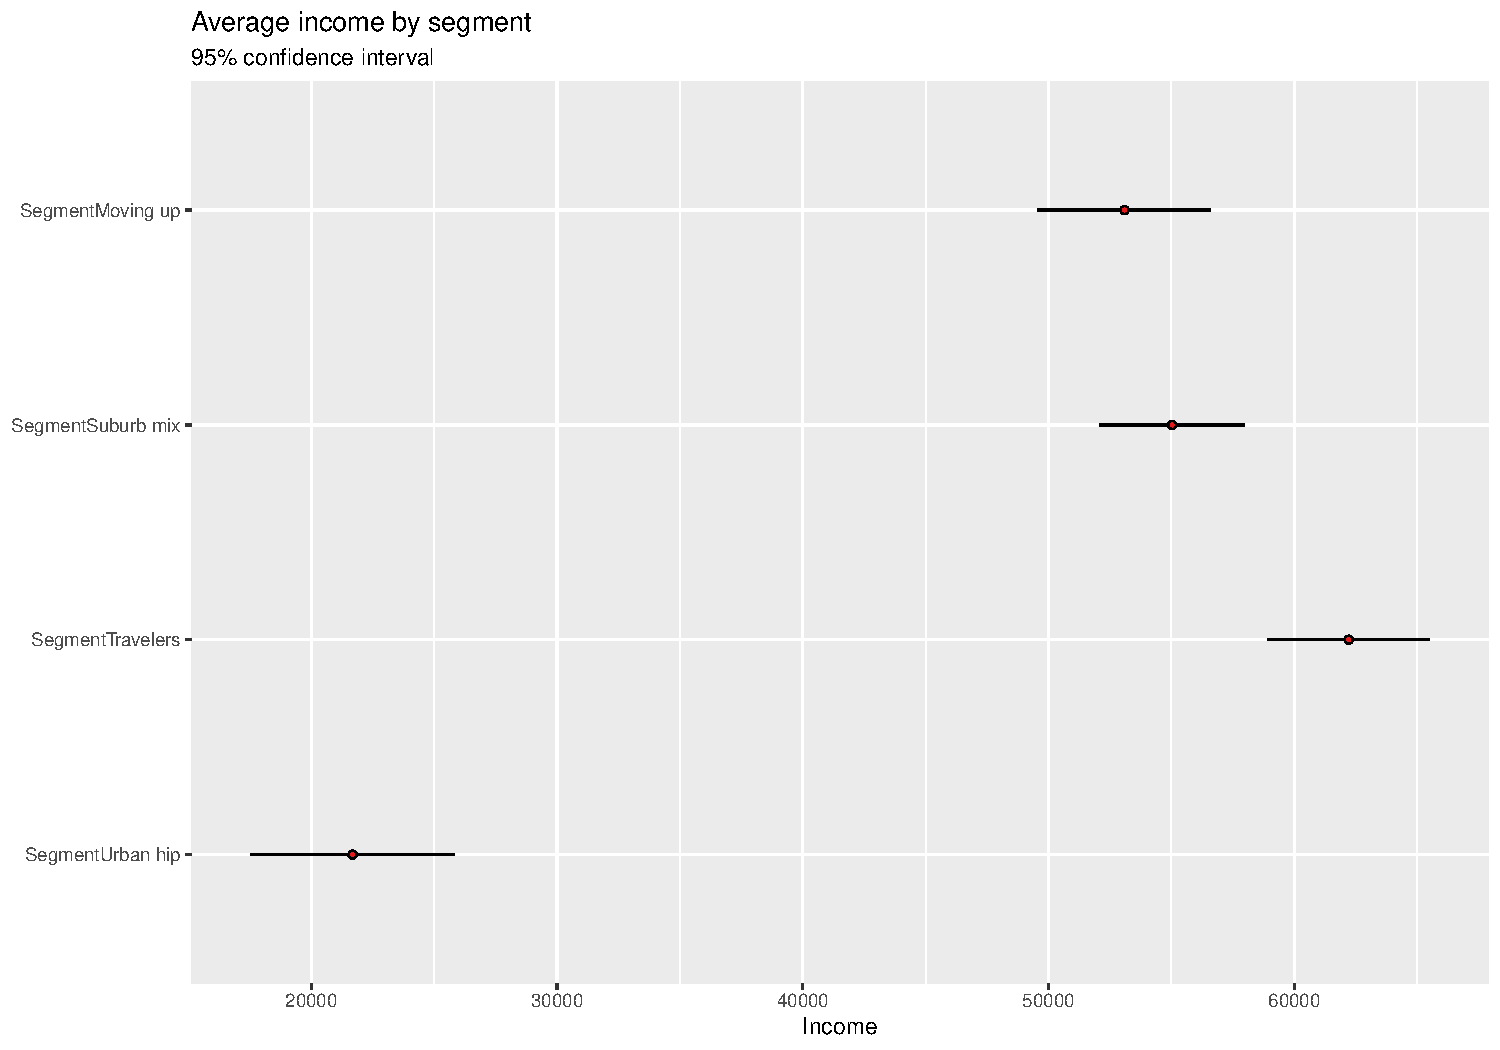
\includegraphics[width=0.85\textwidth,height=\textheight]{006_comparing_groups_statistical_tests_files/figure-beamer/unnamed-chunk-36-1.pdf}
\end{center}
\end{frame}

\section{Acknowledgments}\label{acknowledgments}

\begin{frame}{}
\phantomsection\label{section-40}
\begin{itemize}
\item
  To my family that supports me
\item
  To the taxpayers of Colombia and the
  \href{https://www.umng.edu.co/estudiante}{\textbf{UMNG students}} who
  pay my salary
\item
  To the \href{https://www.business-science.io/}{\textbf{Business
  Science}} and \href{https://www.rfordatasci.com/}{\textbf{R4DS Online
  Learning}} communities where I learn
  \href{https://www.r-project.org/about.html}{\textbf{R}} and
  \href{https://www.python.org/about/}{\textbf{\(\pi\)-thon}}
\item
  To the \href{https://www.r-project.org/contributors.html}{\textbf{R
  Core Team}}, the creators of
  \href{https://posit.co/products/open-source/rstudio/}{\textbf{RStudio
  IDE}}, \href{https://quarto.org/}{\textbf{Quarto}} and the authors and
  maintainers of the packages
  \href{https://CRAN.R-project.org/package=tidyverse}{\textbf{tidyverse}}
  and
  \href{https://CRAN.R-project.org/package=tinytex}{\textbf{tinytex}}
  for allowing me to access these tools without paying for a license
\item
  To the \href{https://www.kernel.org/category/about.html}{\textbf{Linux
  kernel community}} for allowing me the possibility to use some
  \href{https://static.lwn.net/Distributions/}{\textbf{Linux
  distributions}} as my main
  \href{https://en.wikipedia.org/wiki/Operating_system}{\textbf{OS}}
  without paying for a license
\end{itemize}
\end{frame}

\section*{References}\label{references}
\addcontentsline{toc}{section}{References}

\begin{frame}[allowframebreaks]{References}
\phantomsection\label{refs}
\begin{CSLReferences}{1}{0}
\bibitem[\citeproctext]{ref-chapman_r_2019}
Chapman, Chris, and Elea McDonnell Feit. 2019. \emph{R {For} {Marketing}
{Research} and {Analytics}}. 2nd ed. 2019. Use {R}! Cham: Springer
International Publishing : Imprint: Springer.
\url{https://doi-org.ezproxy.umng.edu.co/10.1007/978-3-030-14316-9}.

\end{CSLReferences}
\end{frame}




\end{document}
